% MÉTODOS Y MATERIALES

\cleardoublepage

\chapter{Materiales y métodos}

\section{Materiales}
Seguidamente se enumera todo el material que se ha utilizado para la realización de este trabajo.

\subsection{Datos}
\label{materiales-datos}

En la sección \textbf{Tratamiento de datos}\ref{tratamiento-datos} del capítulo anterior se puede consultar una mención a los dataset que se van a utilizar y que seguidamente se pasan a describir más en profundidad.

\subsubsection{FMA (Free Music Archive) Dataset}

Con un tamaño de más de 100,000 pistas y 160 géneros, se trata de un \emph{dataset} enorme, que cuenta con piezas representativas de cada género. Está respaldado por un repositorio \href{https://github.com/mdeff/fma}{GitHub} que además provee unos \emph{scripts} con ejemplos y algoritmos en \emph{Python}, que extraen información sobre estructura, contenido, organización, etc., del conjunto de datos.

Todas las pistas se encuentran en formato \emph{MP3} (44.1 kHz, 128-320 kbps). Existen tres variantes en cuanto al tamaño del conjunto de datos:

\begin{itemize}
    \item \textbf{FMA Small:} 8,000 pistas, 8 géneros, aproximadamente 1GB.
    \item \textbf{FMA Medium:} 25,000 pistas, 16 géneros, aproximadamente 10GB.
    \item \textbf{FMA Large:} 106,000 pistas, 161 géneros, aproximadamente 100GB. \textbf{(Esta ha sido la variante utilizada).}
\end{itemize}

Se incluyen metadatos como título, artista, álbum, y etiquetas de género. Los géneros musicales están repartidos en niveles de manera jerárquica, siendo los géneros \emph{parent} de primer orden los siguientes:

\begin{multicols}{4}
\begin{itemize}
    \item Blues
    \item Classical
    \item Country
    \item Disco
    \item Hip-Hop
    \item Jazz
    \item Metal
    \item Pop
    \item Reggae
    \item Rock
\end{itemize}
\end{multicols}

\subsubsection{Million Song Dataset}

Se trata de un \emph{dataset vivo}. De base, cuenta con 1500 ficheros en formato \emph{MP3}, distribuidos en 15 categorías de género. Sin embargo, \href{https://www.kaggle.com/datasets/undefinenull/million-song-dataset-spotify-lastfm}{este conjunto de datos} puede hacerse tan grande como se necesite, pues viene acompado de unos ficheros \emph{Python} que realizan una integración con servicios como Spotify y Last.fm. Además de eso, la sincronización con estos dos servicios brinda acceso a metadatos sobre popularidad, características del sonido y etiquetas de géneros.

Así pues, se podría decir que este \emph{dataset} brinda la posibilidad de tener ``toda'' la música de la red disponible para trabajar con ella.

Los géneros de los que se dispone son:
\begin{multicols}{4}
\begin{itemize}
    \item Electronic
    \item Rock
    \item Pop
    \item Folk
    \item Jazz
    \item Blues
    \item Country
    \item Reggae
    \item Latin
    \item R\&B
    \item World
    \item Rap
    \item Punk
    \item New Age
    \item Metal
\end{itemize}
\end{multicols}

\subsubsection{MTG-Jamendo Dataset}

Este \emph{dataset} cuenta con más de 50,000 pistas y 190 géneros, en ficheros \emph{MP3} de 320 kbps . Enorme donde los haya, esta librería fue desarrollada para tareas de etiquetado automático de música. Contiene un conjunto de etiquetas entre las que se encuentran: géneros musicales, instrumentos, emociones y temas. Viene respaldado por un repositorio \href{https://github.com/MTG/mtg-jamendo-dataset}{GitHub} que provee de scripts para su descarga y manejo, así como información sobre su contenido e información estadística.

Los géneros que se pueden encontrar, entre otros, son:
\begin{multicols}{4}
\begin{itemize}
    \item Electronic
    \item Rock
    \item Pop
    \item Folk
    \item Jazz
    \item Hip-Hop
    \item Classical
    \item Reggae
    \item Ska
    \item Swing
    \item Fusion
    \item Easy Listening
    \item Opera
    \item Gospel
    \item Holiday
    \item Comedy
    \item Spoken Word
    \item Podcast
    \item Sound Effects
\end{itemize}
\end{multicols}

Dentro de las modalidades de \emph{dataset} que provee este repositorio, se ha elegido \emph{autotagging\_moodtheme}, que provee ficheros de 30 segundos de duración con etiqueta de género, entre otras.

%python3 scripts/download/download.py --dataset autotagging_moodtheme --type audio  /media/luke/32B841C3B8418677/VIU\ dataset\ mtg/ --unpack

%\subsubsection{Tabla comparativa de tramos entre datasets}
%\begin{table}[h]
\caption{Resumen comparativo de los datasets utilizados}
\centering
\begin{tabular}{|l|l|l|l|}
\hline
\textbf{Dataset} & \textbf{Formato} & \textbf{Volumen} \\ \hline
FMA & MP3 & Hasta 106,000 pistas \\ \hline
Million Song Dataset & MP3 & 1500 (ampliable bajo integración)  \\ \hline
MTG-Jamendo & MP3 & 55,000 pistas \\ \hline
\end{tabular}
\end{table}


\subsection{Software}

Para el desarrollo de este trabajo se han utilizado múltiples y diversos programas, desde el momento en que se inició este mismo documento que ustéd está leyendo, hasta que se produzca la ``puesta en producción'' de la aplicación de usuario que permita el uso del modelo de Inteligencia Artificial.

Los recursos de tipo \emph{Software} utilizados son:

\begin{itemize}
    \item VisualStudio Code. Versión 1.97.2. Entorno de desarrollo de este mismo manual y manejo de datasets y scripts de \emph{Python}.
    \item TextShop. Version 5.49 (5.49). Compilador \LaTeX.
    \item Git. Versión 2.39.3 (Apple Git-145). Gestor de versiones de código fuente para los ficheros de código de este mismo manual y del software desarrollado.
    \item GitHub. Repositorio ``en la nube'' de código fuente.
    \item Draw.io. Editor de diagramas UML.
    \item reMarkable for MacOS. Versión 3.17.0 (906). Software de sincronización del dispositivo reMarkable 2.
    \item Mozilla Firefox. Versión 135.0.1 (64-bit). Explorador de Internet utilizado para el acceso a Jupyter Lab.
    \item Ubuntu 24.04.2 LTS.
    \item Jupyter (Notebook and Lab). Versión 7.2.2.
    \item Python Version: 3.12.7 (major=3, minor=12, micro=7, releaselevel='final', serial=0) | packaged by Anaconda, Inc. | (main, Oct  4 2024, 13:27:36) [GCC 11.2.0]
    \item Librería de Ptyhon \emph{Torch}. Version: 2.6.0+cu124. En el apéndice \ref{apendice-a:paquetes} se pude consultar la lista de todos los paquetes y versiones disponibles para el desarrollo.
    \item CUDA Version: 12.4
    \item cuDNN Version: 90100
    \item NVIDIA Driver Version: 550.127.08
    \item NCCL Version: (2, 21, 5)
\end{itemize}

\subsection{Hardware}

El hardware usado para el desarrollo de este TFM ha sido:

\begin{itemize}
    \item Ordenador \textbf{MacBook Pro 15 pulgadas, 2017.}
    \begin{itemize}
        \item Intel Core i7 2.8 GHz Quad-Core.
        \item 16 GB LPDDR3 2133 MHz.
        \item Intel HD Graphics 630 - Radeon PRO 555 2 GB PCIe.
        \item HD SSD 500 GB.
    \end{itemize}
    \item Ordenador \textbf{Asus ROG Strix G16 G614JIR-N4004 - Gaming 16 pulgadas, 2024.}
    \label{ASUS}
    \begin{itemize}
        \item Intel Core i9-14900HX.
        \item 32 GB LPDDR3 2133 MHz.
        \item NVIDIA RTX 4070 8GB Mobile.
        \item HD SSD 1 TB.
    \end{itemize}
    \item Paper tablet \textbf{reMarkable 2.}
\end{itemize}

Dada la filia y el vicio de uso con el sistema operativo de Apple, se ha utilizado un Apple MacBook Pro para todo el proceso de escritura de documentación y como terminal de programación, siendo usado como interfaz con el otro ordenador ASUS, usado como nodo de procesamiento para el entrenamiento de los modelos de Inteligencia Artificial.

En las referencias \cite{geeksforgeeks2025jupyter} y \cite{vscode2025jupyter} se puede consultar cómo se ha configurado el ``servidor de procesamiento'' basado en \emph{Jupyter Lab}, instalado en la máquina ASUS\ref{ASUS}, en un Sistema Operativo Ubuntu 24.04.2 LTS.

En la imagen \ref{fig:jupyter-diagram} se pude ver un diagrama de cuáles son los accesos posible que brinda el servidor Jupyter para poder ejecutar el código Python de un situado en un ordenador, desde otro; o para poder directamente ejecutar el código Python situado en un ordenador (MacBook), en otra máquina distinta (ASUS), instanciando el entorno Python de esta otra máquina, a través del puerto configurado.

\begin{figure}[H]
\centering
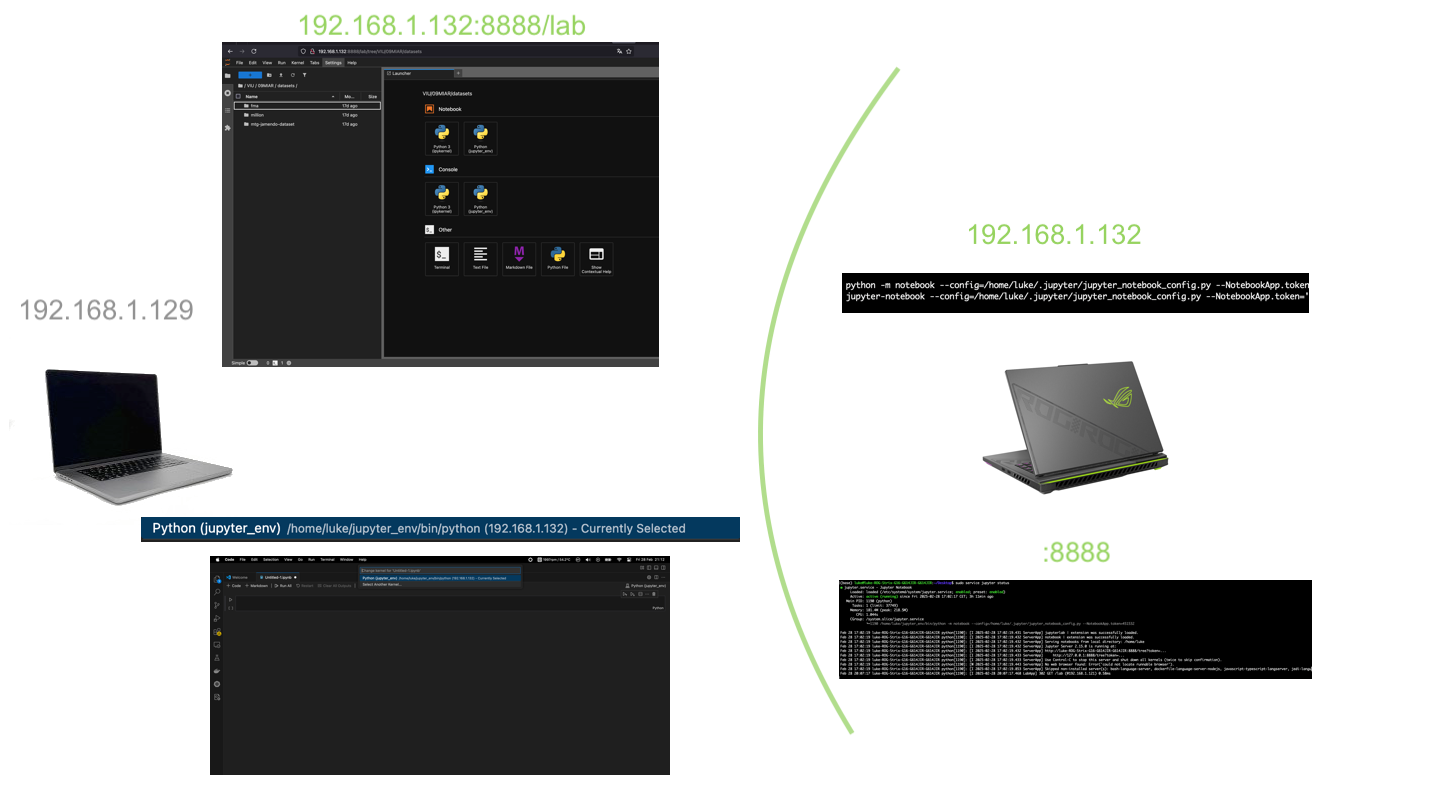
\includegraphics[width=0.9\textwidth]{images/jupyter-diagram.png}
\caption{Diagrama de conexión hardware.}
\label{fig:jupyter-diagram}
\end{figure}

Jupyter Lab estará esperando detrás del puerto 8888 de la máquina ASUS, la cual podrá ser instanciada por VistualStudio Code como Jupyter kernel o ser accesible vía explorador de Internet, pudiendo usar el entorno de edición y ejecución web que el servicio provee.

De esta manera se consigue usar toda la potencia de una máquina, desde la comodidad de uso y cercanía que brinda la otra.

\section{Metodología}

Para el desarrollo de este TFM y del software que lo culminará, se han barajado 3 maneras, \emph{frameworks} o métodos de emprender y encaminar esta labor, de manera rigurosa, estructurada y ordenada. Los nombres que se han manejado han sido:
\begin{itemize}
    \item CRSIP-ML(Q): Cross Industry Standard Process for Machine Learning with Quality Assurance
    \item TDSP: Team Data Science Process
    \item Scrum: del rugby, ideal que significa trabajo en equipo y rápida respuesta de adaptación.
\end{itemize}

Cada una de estas tres herramientas aporta valor a cada uno de los pasos que se puedan llevar a cabo. Haciendo un análisis más profundo y tal y como se explica en la entrada web\cite{TDSP-PM}, se podría decir que \emph{TDSP} podría ser la combinación de \emph{Scrum} y \emph{CRISP-DM} (Cross Industry Standard Process for Data Mining. En el caso de proyectos de Machine Learning, CRISP-ML(Q) parte de la misma filosfía y se adapta a las necesidades específicas de este tipo de trabjos). Así pues, dado que todo lo referente a gestión de equipo y recursos en paralelo es innecesario, pues este trabajo se realiza por una sola persona, se ha decidido tomar un combinación de \textbf{CRISP-ML(Q)} y \textbf{Scrum}, que permita ser tan riguroso como el primero de ellos y tan ágil y potente en cuanto a herramientas, como el segundo.

\subsection{CRISP-ML(Q)}

\begin{figure}[H]
    \centering
    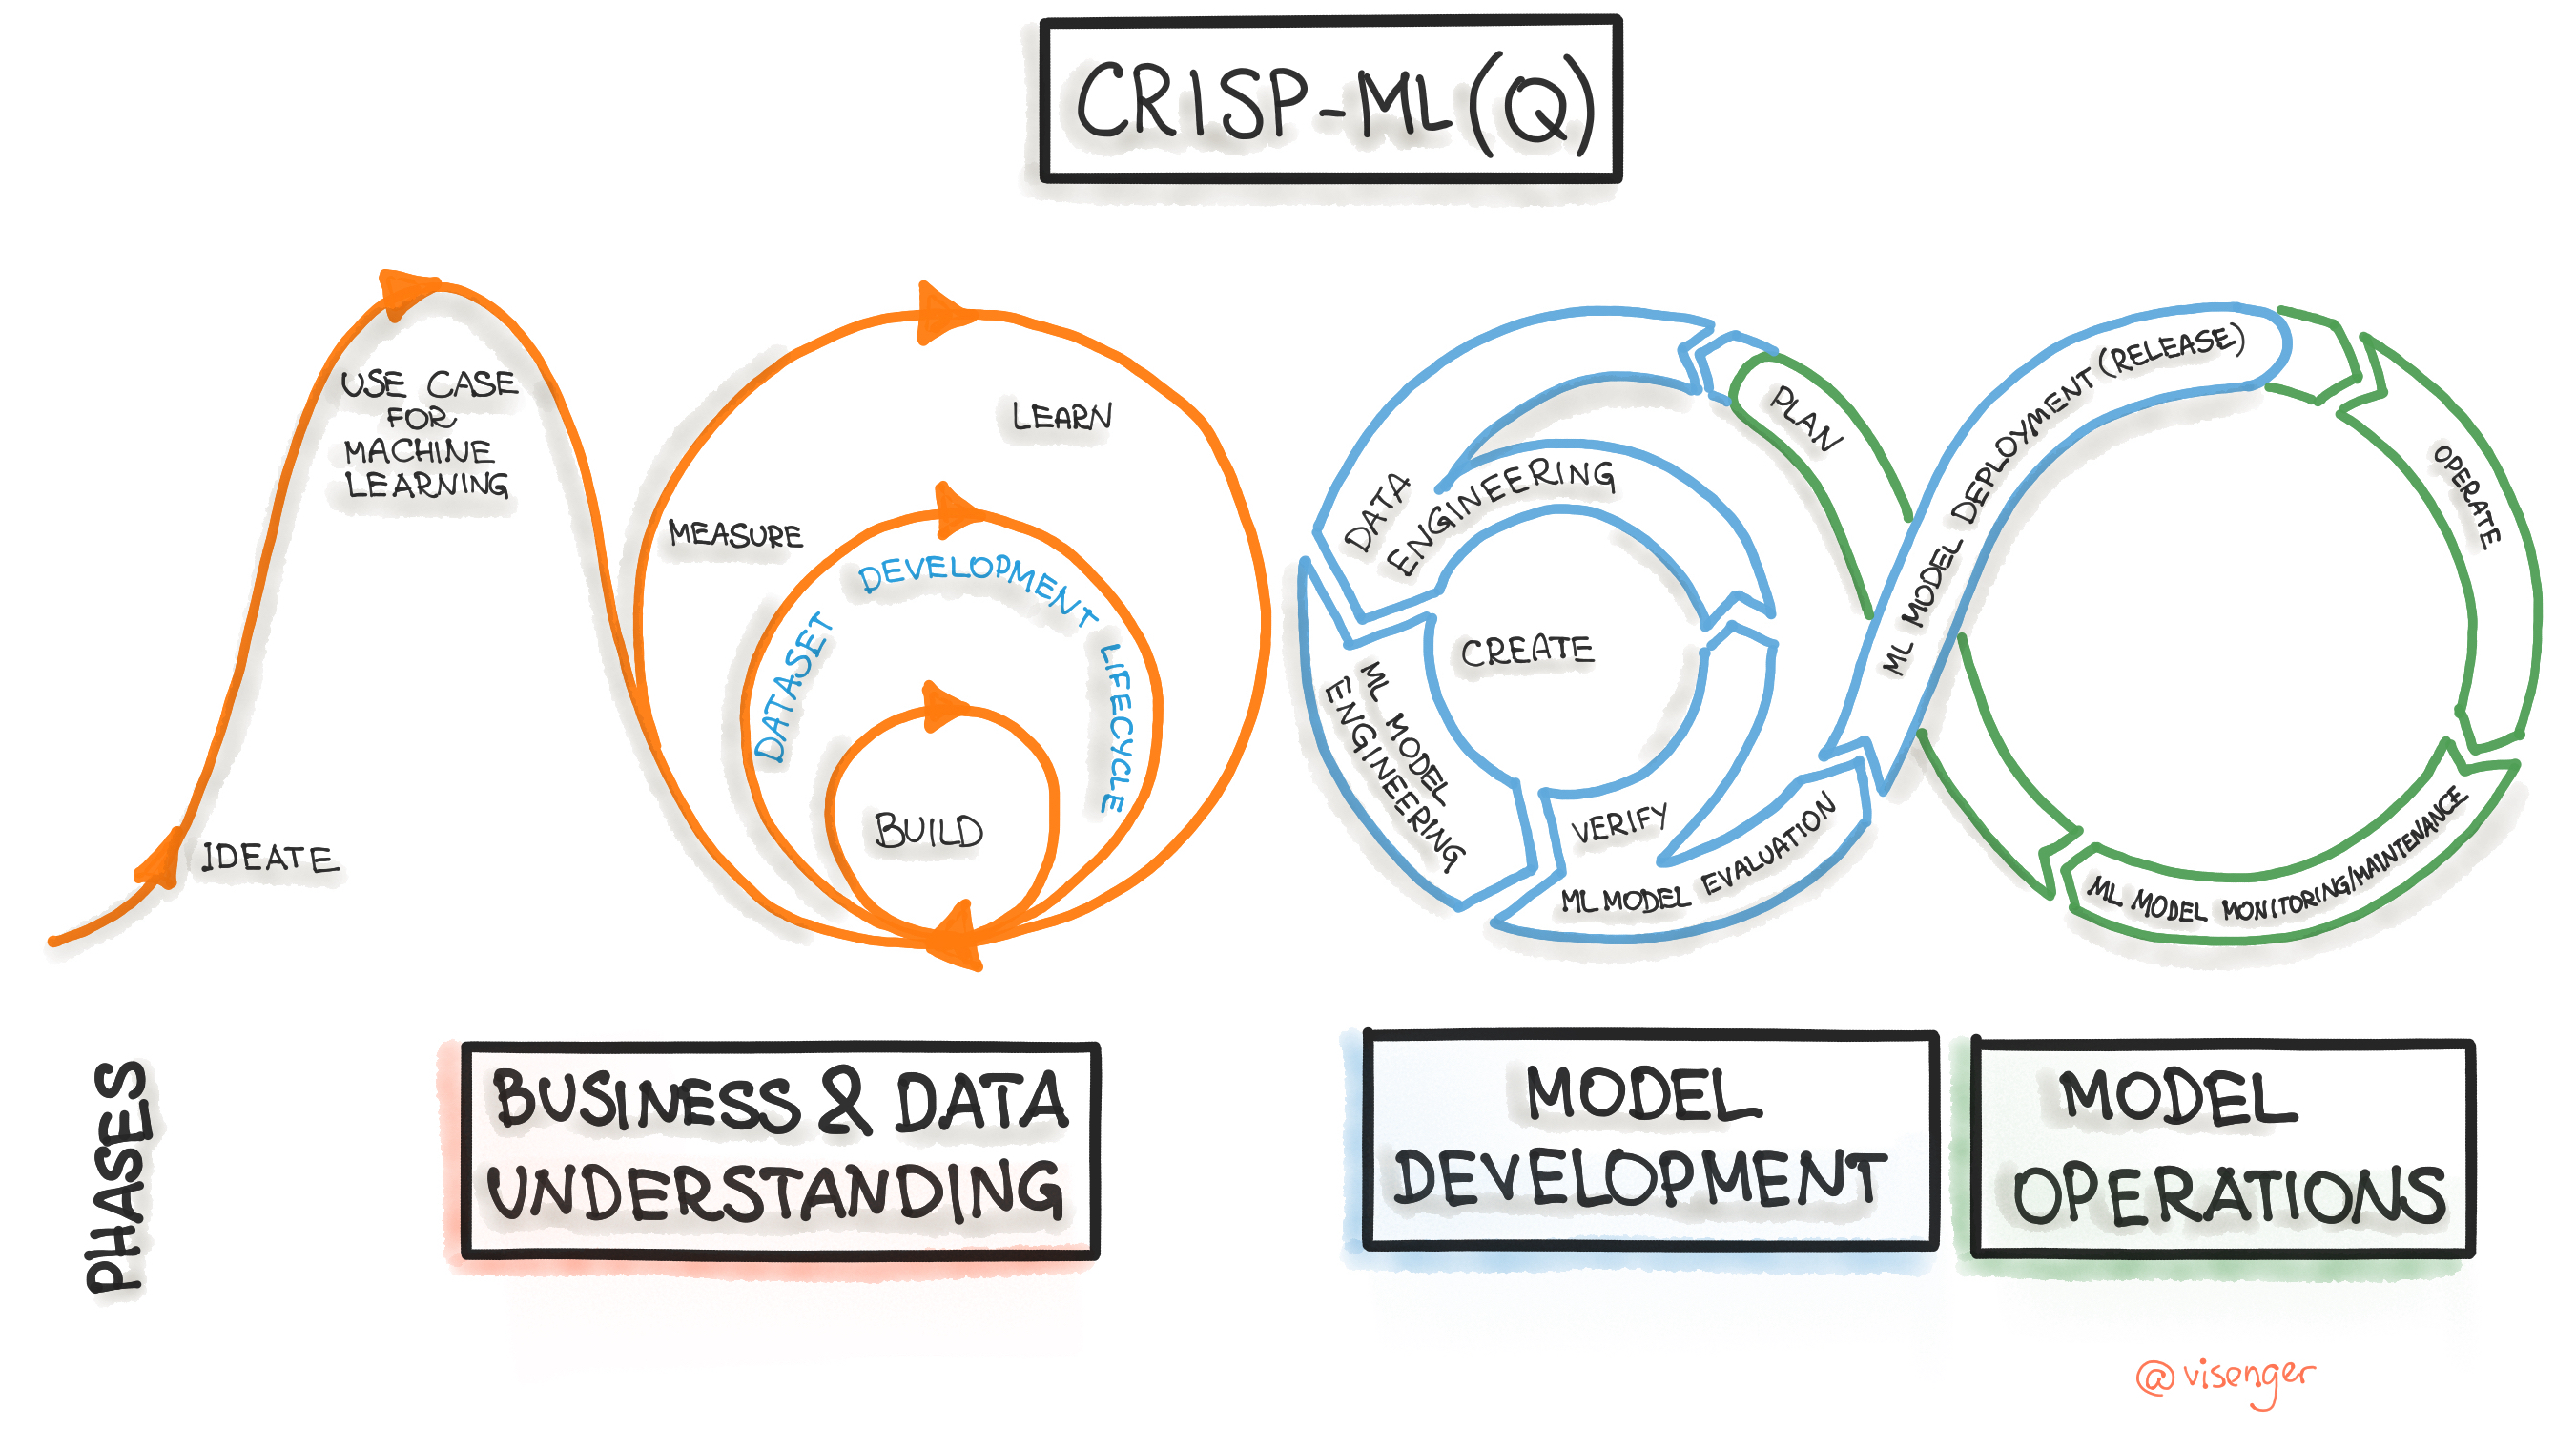
\includegraphics[width=0.9\textwidth]{images/crisp-ml-process.jpg}
    \caption{Diagrama de flujo usado en el desarrollo. Tomado de \cite{crispml}.}
    \label{fig:crispml-q-diagram}
  \end{figure}

\emph{CRISP-ML(Q)} conforma un marco estructurado para el desarrollo de proyectos de Machine Learning. Se compone de seis fases:

\begin{enumerate}
    \item \textbf{Comprensión del negocio}: Definir el problema y los objetivos del modelo.
    \item \textbf{Comprensión de los datos}: Recopilación y exploración inicial de los datos.
    \item \textbf{Preparación de los datos}: Limpieza, transformación y selección de variables.
    \item \textbf{Modelado}: Entrenamiento y optimización de modelos de Machine Learning.
    \item \textbf{Evaluación}: Validación de métricas y análisis del rendimiento.
    \item \textbf{Implementación y monitoreo}: Despliegue del modelo y seguimiento en producción.
\end{enumerate}

En la imagen\ref{fig:crispml-q-diagram} se puede ver cómo será el diagrama de flujo del desarrollo a seguir con este método.

\subsection{Scrum}

\emph{Scrum} es un framework que proporciona herramientas para la gestión ágil de proyectos de manera iterativa, dividiendo el trabajo en sprints (iteraciones cortas de 1-2 semanas). Las herramientas de \emph{Scrum} que se tomen para este proyecto serán:

\begin{itemize}
    \item \textbf{Product Backlog}: Lista priorizada de tareas a realizar.
    \item \textbf{Sprints}: Iteraciones donde se completan tareas específicas. Semanales.
    \item \textbf{Sprint Reviews}: Evaluaciones de cada sprint (semana o bisemanal) con la tutora de este TFM.
\end{itemize}

\subsection{Integración de CRISP-ML(Q) y Scrum}

A continuación, se detalla la planificación del TFM en base a estos marcos metodológicos.

\subsection{Product Backlog (Pila de producto)}

Las tareas que se han de llevar a cabo para completar el TFM, incluidos desarrollo de la documentación, software y evaluación y mantenimiento, se han organizado en el siguiente \emph{backlog}:

% \begin{table}[h]
%     \centering
    
%     \resizebox{\textwidth}{!}{
%     \begin{tabular}{|c|c|p{8cm}|c|}
%         \hline
%         \textbf{Épica} & \textbf{Historia de Usuario} & \textbf{Tareas} & \textbf{Prioridad} \\
%         \hline
%         Comprensión del negocio & Definir el problema & Redactar introducción, revisar 10 artículos, definir impacto y KPIs & Alta \\
%         \hline
%         Comprensión de los datos & Analizar calidad de los datos & Inspeccionar valores nulos, outliers, generar gráficos EDA & Alta \\
%         \hline
%         Preparación de los datos & Preprocesamiento de datos & Normalizar, codificar variables, dividir en train/test & Media \\
%         \hline
%         Modelado & Entrenar modelos de ML & Implementar baseline, probar algoritmos, ajustar hiperparámetros & Alta \\
%         \hline
%         Evaluación & Validar rendimiento del modelo & Comparar métricas, generar reportes de resultados & Alta \\
%         \hline
%         Implementación y monitoreo & Redactar el TFM & Documentar metodología, resultados, preparar presentación & Alta \\
%         \hline
%     \end{tabular}}
% \end{table}

\begin{table}[h]
    \centering
    \caption{Product Backlog (Pila de producto) del TFM basado en CRISP-ML(Q) y Scrum}
    \resizebox{0.8\textwidth}{!}{
    \begin{tabular}{|c|p{8cm}|p{8cm}|}
        \hline
        \textbf{Épica (Fase CRISP-ML(Q))} & \textbf{Historia de Usuario} & \textbf{Tareas} \\
        \hline
        Comprensión del negocio &  Como estudiante, quiero comprender bien el problema para entender el alcance del proyecto. & 
        \begin{itemize}
            \item Redactar introducción.
            \item Definir objetivos generales y específicos.
            \item Entender y tomar notas sobre el alcance del proyecto.
        \end{itemize} \\
        \hline
        Comprensión del negocio & Como estudiante, en mi labor de investigación, quiero revisar literatura existente en torno al problema.  &
        \begin{itemize}
            \item Buscar y analizar artículos y publicaciones relevantes. 
            \item Extraer ideas clave.
            \item Identificar tendencias en el estado del arte.
        \end{itemize} \\
        \hline
        Comprensión de los datos & Como estudiante, emulando a un científico de datos, quiero inspeccionar los datos disponibles para evaluar su calidad. & 
        \begin{itemize}
            \item Encontrar fuentes con datasets adecuados.
            \item Revisar estructura y tipos de datos.
            \item Evaluar insuficiencia, sesgo o desbalanceo en los datos.
            \item Escribir la metodología detallada.
        \end{itemize} \\
        \hline
        Preparación de los datos & Como estudiante y desarrollador, quiero limpiar y transformar los datos para que sean aptos para el modelo. & 
        \begin{itemize}
            \item Normalizar y codificar variables.
            \item Manejar valores atípicos y nulos.
        \end{itemize} \\
        \hline
        Preparación de los datos & Como estudiante y desarrollador, quiero dividir los datos en conjuntos de entrenamiento, validación y prueba. & 
        \begin{itemize}
            \item Definir proporción de separación de datos.
            \item Verificar balanceo de clases.
        \end{itemize} \\
        \hline
        Modelado & Como estudiante, emulando a un científico de datos, quiero entrenar un modelo base para establecer un punto de comparación. & 
        \begin{itemize}
            \item Entrenar el VAE.
            \item Evaluar rendimiento inicial.
            \item Extraer los primeros resultados.
        \end{itemize} \\
        \hline
        Modelado & Como estudiante, emulando a un científico de datos, quiero entrenar un modelo basado en GAN-Transformer y evaluar su precisión. & 
        \begin{itemize}
            \item Implementar y entrenar el modelo GAN-Transformer.
            \item Comparar modelos con métricas clave.
        \end{itemize} \\
        \hline
        Evaluación & Como estudiante e investigador, quiero evaluar el rendimiento del modelo para justificar su efectividad. &
        \begin{itemize}
            \item Calcular precisión, recall y F1-score.
            \item Generar matriz de confusión.
            \item Comparar modelos.
        \end{itemize} \\
        \hline
        Evaluación & Como estudiante e investigador, quiero establecer métricas comparativas entre los enfoques y mejorar la red GAN. & 
        \begin{itemize}
            \item Analizar interpretabilidad de los resultados.
            \item Ajustar hiperparámetros y arquitectura.
        \end{itemize} \\
        \hline
        Implementación y monitoreo & Como estudiante, quiero documentar la metodología utilizada para su presentación y evaluación. & 
        \begin{itemize}
            \item Documentar pruebas de los modelos.
            \item Preparar informe técnico.
        \end{itemize} \\
        \hline
        Implementación y monitoreo & Como estudiante, quiero preparar una presentación clara y concisa para la defensa del TFM. & 
        \begin{itemize}
            \item Diseñar diapositivas con gráficos y métricas.
            \item Exponer conclusiones.
            \item Practicar la presentación.
        \end{itemize} \\
        \hline
    \end{tabular}}
\end{table}


\clearpage
\begin{tcolorbox}[colback=black!85!white, colframe=orange!60!black, fontupper=\color{white},
    title=\textbf{\huge Product Backlog (Pila de producto)}, fonttitle=\color{white}]
    
        \begin{center}
        \renewcommand{\arraystretch}{0.2} % Reduce la separación entre filas
        \setlength{\tabcolsep}{8pt} % Reduce la separación entre columnas
        \resizebox{0.8\textwidth}{!}{ % Ajusta la tabla al 95% del ancho del texto
        \begin{tabular}{m{0.32\textwidth}<{\raggedright} m{0.32\textwidth}<{\raggedright} m{0.32\textwidth}<{\raggedright}} % 3 COLUMNAS BALANCEADAS
        
            %%%% FILA 1 - Comprensión del negocio (CN)
            \begin{tcolorbox}[colback=yellow!70!white, colframe=yellow!90!white, title={\textbf{CN-1}}, fonttitle=\color{black}]
            Redactar introducción.
            \end{tcolorbox} &        
            \begin{tcolorbox}[colback=yellow!70!white, colframe=yellow!90!white, title={\textbf{CN-2}}, fonttitle=\color{black}]
            Definir objetivos generales y específicos.
            \end{tcolorbox} &        
            \begin{tcolorbox}[colback=yellow!70!white, colframe=yellow!90!white, title={\textbf{CN-3}}, fonttitle=\color{black}]
            Entender y tomar notas sobre el alcance del proyecto.
            \end{tcolorbox} \\
    
            %%%% FILA 2
            \begin{tcolorbox}[colback=yellow!70!white, colframe=yellow!90!white, title={\textbf{CN-4}}, fonttitle=\color{black}]
            Buscar y analizar artículos y publicaciones relevantes.
            \end{tcolorbox} &
            \begin{tcolorbox}[colback=yellow!70!white, colframe=yellow!90!white, title={\textbf{CN-5}}, fonttitle=\color{black}]
            Extraer ideas clave.
            \end{tcolorbox} &
            \begin{tcolorbox}[colback=yellow!70!white, colframe=yellow!90!white, title={\textbf{CN-6}}, fonttitle=\color{black}]
            Identificar tendencias en el estado del arte.
            \end{tcolorbox} \\
    
            %%%% FILA 3 - Comprensión de los datos (CD)
            \begin{tcolorbox}[colback=purple!30!white, colframe=purple!40!white, title={\textbf{CD-1}}, fonttitle=\color{black}]
            Encontrar fuentes con datasets adecuados.
            \end{tcolorbox} &
            \begin{tcolorbox}[colback=purple!30!white, colframe=purple!40!white, title={\textbf{CD-2}}, fonttitle=\color{black}]
            Revisar estructura y tipos de datos.
            \end{tcolorbox} &
            \begin{tcolorbox}[colback=purple!30!white, colframe=purple!40!white, title={\textbf{CD-3}}, fonttitle=\color{black}]
            Evaluar insuficiencia, sesgo o desbalanceo en los datos.
            \end{tcolorbox} \\
    
            %%%% FILA 4
            \begin{tcolorbox}[colback=purple!30!white, colframe=purple!40!white, title={\textbf{CD-4}}, fonttitle=\color{black}]
            Escribir la metodología detallada.
            \end{tcolorbox} &
            \begin{tcolorbox}[colback=green!50!yellow, colframe=green!80!yellow, title={\textbf{PD-1}}, fonttitle=\color{black}]
            Normalizar y codificar variables.
            \end{tcolorbox} &
            \begin{tcolorbox}[colback=green!50!yellow, colframe=green!80!yellow, title={\textbf{PD-2}}, fonttitle=\color{black}]
            Manejar valores atípicos y nulos.
            \end{tcolorbox} \\
            \begin{tcolorbox}[colback=green!50!yellow, colframe=green!80!yellow, title={\textbf{PD-3}}, fonttitle=\color{black}]
            Definir proporción de separación de datos.
            \end{tcolorbox} &
    
            %%%% FILA 5
            \begin{tcolorbox}[colback=green!50!yellow, colframe=green!80!yellow, title={\textbf{PD-4}}, fonttitle=\color{black}]
            Verificar balanceo de clases.
            \end{tcolorbox} &
            \begin{tcolorbox}[colback=pink!60!red, colframe=pink!40!red, title={\textbf{M-1}}, fonttitle=\color{black}]
            Entrenar el VAE.
            \end{tcolorbox} \\
            \begin{tcolorbox}[colback=pink!60!red, colframe=pink!40!red, title={\textbf{M-2}}, fonttitle=\color{black}]
            Evaluar rendimiento inicial.
            \end{tcolorbox} &
    
            %%%% FILA 6
            \begin{tcolorbox}[colback=pink!60!red, colframe=pink!40!red, title={\textbf{M-3}}, fonttitle=\color{black}]
            Extraer los primeros resultados.
            \end{tcolorbox} &
            \begin{tcolorbox}[colback=pink!60!red, colframe=pink!40!red, title={\textbf{M-4}}, fonttitle=\color{black}]
            Implementar y entrenar el modelo GAN-Transformer.
            \end{tcolorbox} \\
            
            \begin{tcolorbox}[colback=pink!60!red, colframe=pink!40!red, title={\textbf{M-5}}, fonttitle=\color{black}]
            Comparar modelos con métricas clave.
            \end{tcolorbox} &
            \begin{tcolorbox}[colback=orange!70!white, colframe=orange!90!white, title={\textbf{EV-1}}, fonttitle=\color{black}]
            Calcular precisión, recall y F1-score.
            \end{tcolorbox} &
            \begin{tcolorbox}[colback=orange!70!white, colframe=orange!90!white, title={\textbf{EV-2}}, fonttitle=\color{black}]
            Generar matriz de confusión.
            \end{tcolorbox}
            \\

            %%%% FILA 8
            \begin{tcolorbox}[colback=orange!70!white, colframe=orange!90!white, title={\textbf{EV-3}}, fonttitle=\color{black}]
                Comparar modelos.
                
                \end{tcolorbox}
            &
            
            \begin{tcolorbox}[colback=orange!70!white, colframe=orange!90!white, title={\textbf{EV-4}}, fonttitle=\color{black}]
                Analizar interpretabilidad de los resultados.
                \end{tcolorbox} &

                \begin{tcolorbox}[colback=orange!70!white, colframe=orange!90!white, title={\textbf{EV-5}}, fonttitle=\color{black}]
                    Ajustar hiperparámetros y arquitectura.
                    \end{tcolorbox} 

            \\
    
            %%%% FILA 9
            
            \begin{tcolorbox}[colback=blue!30!white, colframe=blue!40!white, title={\textbf{IM-1}}, fonttitle=\color{black}]
            Documentar pruebas de los modelos.
            \end{tcolorbox} &
            \begin{tcolorbox}[colback=blue!30!white, colframe=blue!40!white, title={\textbf{IM-2}}, fonttitle=\color{black}]
            Preparar informe técnico.
            \end{tcolorbox} &
    
            %%%% FILA 10
            \begin{tcolorbox}[colback=blue!30!white, colframe=blue!40!white, title={\textbf{IM-3}}, fonttitle=\color{black}]
            Diseñar diapositivas con gráficos y métricas.
            \end{tcolorbox} \\
            \begin{tcolorbox}[colback=blue!30!white, colframe=blue!40!white, title={\textbf{IM-4}}, fonttitle=\color{black}]
            Exponer conclusiones.
            \end{tcolorbox} &
            \begin{tcolorbox}[colback=blue!30!white, colframe=blue!40!white, title={\textbf{IM-5}}, fonttitle=\color{black}]
            Practicar la presentación.
            \end{tcolorbox} \\
    
        \end{tabular}
        }
        \end{center}
    
    \end{tcolorbox}
    
\clearpage
% \begin{table}[h]
    \centering
    \caption{Estado ``actual'' de progreso del TFM basado en CRISP-ML(Q) y Scrum}
    \resizebox{\textwidth}{!}{
    \begin{tabular}{|p{8cm}|c|p{2.5cm}|}
        \hline
        \textbf{Tarea} & \textbf{Categoría\hfill \break CRISP-ML(Q) / (Código)} & \textbf{Estado} \\
        \hline
        Redactar introducción & Comprensión del negocio / (CN-1) & \ding{51}Hecho \\
        \hline
        Definir objetivos generales y específicos & Comprensión del negocio / (CN-2) & \ding{51}Hecho \\
        \hline
        Entender y tomar notas sobre el alcance del proyecto & Comprensión del negocio / (CN-3) & \ding{51}Hecho \\
        \hline
        Buscar y analizar artículos y publicaciones relevantes & Comprensión del negocio / (CN-4) & \ding{51}Hecho \\
        \hline
        Extraer ideas clave & Comprensión del negocio / (CN-5) & \ding{51}Hecho \\
        \hline
        Identificar tendencias en el estado del arte & Comprensión del negocio / (CN-6) & \ding{51}Hecho \\
        \hline
        Encontrar fuentes con datasets adecuados & Comprensión de los datos / (CD-1) & \ding{51}Hecho \\
        \hline
        Revisar estructura y tipos de datos & Comprensión de los datos / (CD-2) & \ding{51}Hecho \\
        \hline
        Evaluar insuficiencia, sesgo o desbalanceo en los datos & Comprensión de los datos / (CD-3) & \ding{45}En progreso \\
        \hline
        Escribir la metodología detallada & Implementación y monitoreo / (CD-4) & \ding{51}Hecho \\
        \hline
        Normalizar y codificar variables & Preparación de los datos / (PD-1) & \ding{43}Por hacer \\
        \hline
        Manejar valores atípicos y nulos & Preparación de los datos / (PD-2) & \ding{43}Por hacer \\
        \hline
        Definir proporción de separación de datos & Preparación de los datos / (PD-3) & \ding{43}Por hacer \\
        \hline
        Verificar balanceo de clases & Preparación de los datos / (PD-4) & \ding{43}Por hacer \\
        \hline
        Entrenar el VAE & Modelado / (M-1) & \ding{43}Por hacer \\
        \hline
        Evaluar rendimiento inicial & Modelado / (M-2) & \ding{43}Por hacer \\
        \hline
        Extraer los primeros resultados & Modelado / (M-3) & \ding{43}Por hacer \\
        \hline
        Implementar y entrenar el modelo GAN-Transformer & Modelado / (M-4) & \ding{43}Por hacer \\
        \hline
        Comparar modelos con métricas clave & Modelado / (M-5) & \ding{43}Por hacer \\
        \hline
        Analizar interpretabilidad de los resultados & Evaluación / (EV-1) & \ding{43}Por hacer \\
        \hline
        Calcular precisión, recall y F1-score & Evaluación / (EV-2) & \ding{43}Por hacer \\
        \hline
        Generar matriz de confusión & Evaluación / (EV-3) & \ding{43}Por hacer \\
        \hline
        Comparar modelos & Evaluación / (EV-4) & \ding{43}Por hacer \\
        \hline
        Ajustar hiperparámetros y arquitectura & Evaluación / (EV-5) & \ding{43}Por hacer \\
        \hline
        Documentar pruebas de los modelos & Implementación y monitoreo / (IM-1) & \ding{43}Por hacer \\
        \hline
        Preparar informe técnico & Implementación y monitoreo / (IM-2) & \ding{43}Por hacer \\
        \hline
        Diseñar diapositivas con gráficos y métricas & Implementación y monitoreo / (IM-3) & \ding{43}Por hacer \\
        \hline
        Exponer conclusiones & Implementación y monitoreo / (IM-4) & \ding{43}Por hacer \\
        \hline
        Practicar la presentación & Implementación y monitoreo / (IM-5) & \ding{43}Por hacer \\
        \hline
    \end{tabular}}
\end{table}

Estableciendo las ``rondas'' iterables de progreso en \emph{sprints} de Scrum, el siguiente \emph{kanban} ilustra el estado ``actual'' del progreso de este trabajo:
\begin{tcolorbox}[colback=black!85!white, colframe=orange!60!black, fontupper=\color{white},
    title=\textbf{\huge Kanban}, fonttitle=\color{white}]
    {\huge \emph{Sprint 3}}
        \begin{center}
            \renewcommand{\arraystretch}{0.2} % Reduce la separación entre filas
            \setlength{\tabcolsep}{8pt} % Reduce la separación entre columnas
            \resizebox{\textwidth}{!}{ % Ajusta la tabla al 95% del ancho del texto
            \begin{tabular}{m{4cm} m{4cm} m{4cm} m{4cm} m{4cm}}
            \begin{center}
            {\Fontauri \huge \emph{to do}}
            \end{center}
            & \begin{center}
            {\Fontauri \huge \emph{to do}} 
            \end{center}
            & \begin{center}
            {\Fontauri \huge \emph{to do}} 
            \end{center}
            & \begin{center}
            {\Fontauri \huge \emph{in progress}} 
            \end{center} 
            & \begin{center}
            {\Fontauri \huge \emph{done}} 
            \end{center} \\
            
            \begin{tcolorbox}[colback=green!50!white, colframe=green!80!black, title={\textbf{PD-1}}, fonttitle=\color{black}]
            Normalizar y codificar variables.
            \end{tcolorbox} &
            \begin{tcolorbox}[colback=green!50!white, colframe=green!80!black, title={\textbf{PD-2}}, fonttitle=\color{black}]
            Manejar valores atípicos y nulos.
            \end{tcolorbox} &
            \begin{tcolorbox}[colback=green!50!white, colframe=green!80!black, title={\textbf{PD-3}}, fonttitle=\color{black}]
            Definir proporción de separación de datos.
            \end{tcolorbox} &
            \begin{tcolorbox}[colback=purple!30!white, colframe=purple!40!white, title={\textbf{CD-3}}, fonttitle=\color{black}]
            Evaluar insuficiencia, sesgo o desbalanceo en los datos.
            \end{tcolorbox} &
            \begin{tcolorbox}[colback=yellow!70!white, colframe=yellow!90!white, title={\textbf{CN-1}}, fonttitle=\color{black}]
            Redactar introducción.
            \end{tcolorbox}
            \\

            \begin{tcolorbox}[colback=green!50!white, colframe=green!80!black, title={\textbf{PD-4}}, fonttitle=\color{black}]
            Verificar balanceo de clases.
            \end{tcolorbox} &
            \begin{tcolorbox}[colback=pink!60!red, colframe=pink!40!red, title={\textbf{M-1}}, fonttitle=\color{black}]
            Entrenar el VAE.
            \end{tcolorbox} &
            \begin{tcolorbox}[colback=pink!60!red, colframe=pink!40!red, title={\textbf{M-2}}, fonttitle=\color{black}]
            Evaluar rendimiento inicial.
            \end{tcolorbox} &
            &
            \begin{tcolorbox}[colback=yellow!70!white, colframe=yellow!90!white, title={\textbf{CN-2}}, fonttitle=\color{black}]
            Definir objetivos generales y específicos.
            \end{tcolorbox}
            \\
            
            \begin{tcolorbox}[colback=pink!60!red, colframe=pink!40!red, title={\textbf{M-3}}, fonttitle=\color{black}]
            Extraer los primeros resultados.
            \end{tcolorbox} & 
            \begin{tcolorbox}[colback=pink!60!red, colframe=pink!40!red, title={\textbf{M-4}}, fonttitle=\color{black}]
            Implementar y entrenar el modelo GAN-Transformer.
            \end{tcolorbox} &
            \begin{tcolorbox}[colback=pink!60!red, colframe=pink!40!red, title={\textbf{M-5}}, fonttitle=\color{black}]
            Comparar modelos con métricas clave.
            \end{tcolorbox} &
            & 
            \begin{tcolorbox}[colback=yellow!70!white, colframe=yellow!90!white, title={\textbf{CN-3}}, fonttitle=\color{black}]
            Entender y tomar notas sobre el alcance del proyecto.
            \end{tcolorbox} 
            \\

            \begin{tcolorbox}[colback=orange!70!white, colframe=orange!90!white, title={\textbf{EV-1}}, fonttitle=\color{black}]
            Analizar interpretabilidad de los resultados.
            \end{tcolorbox} & 
            \begin{tcolorbox}[colback=orange!70!white, colframe=orange!90!white, title={\textbf{EV-2}}, fonttitle=\color{black}]
            Calcular precisión, recall y F1-score.
            \end{tcolorbox} &
            \begin{tcolorbox}[colback=orange!70!white, colframe=orange!90!white, title={\textbf{EV-3}}, fonttitle=\color{black}]
            Generar matriz de confusión.
            \end{tcolorbox} &
            &
            \begin{tcolorbox}[colback=yellow!70!white, colframe=yellow!90!white, title={\textbf{CN-4}}, fonttitle=\color{black}]
            Buscar y analizar artículos y publicaciones relevantes.
            \end{tcolorbox}    
            \\
    
            
            \begin{tcolorbox}[colback=orange!70!white, colframe=orange!90!white, title={\textbf{EV-4}}, fonttitle=\color{black}]
            Comparar modelos.
            \end{tcolorbox} &
            \begin{tcolorbox}[colback=orange!70!white, colframe=orange!90!white, title={\textbf{EV-5}}, fonttitle=\color{black}]
            Ajustar hiperparámetros y arquitectura.
            \end{tcolorbox} &
            \begin{tcolorbox}[colback=blue!30!white, colframe=blue!40!white, title={\textbf{IM-1}}, fonttitle=\color{black}]
            Documentar pruebas de los modelos.
            \end{tcolorbox} &
            &
            \begin{tcolorbox}[colback=yellow!70!white, colframe=yellow!90!white, title={\textbf{CN-5}}, fonttitle=\color{black}]
            Extraer ideas clave.
            \end{tcolorbox} 
            \\
            
            \begin{tcolorbox}[colback=blue!30!white, colframe=blue!40!white, title={\textbf{IM-2}}, fonttitle=\color{black}]
            Preparar informe técnico.
            \end{tcolorbox} &
            \begin{tcolorbox}[colback=blue!30!white, colframe=blue!40!white, title={\textbf{IM-3}}, fonttitle=\color{black}]
            Diseñar diapositivas con gráficos y métricas.
            \end{tcolorbox} &
            \begin{tcolorbox}[colback=blue!30!white, colframe=blue!40!white, title={\textbf{IM-4}}, fonttitle=\color{black}]
            Exponer conclusiones.
            \end{tcolorbox} &
            &
            \begin{tcolorbox}[colback=yellow!70!white, colframe=yellow!90!white, title={\textbf{CN-6}}, fonttitle=\color{black}]
            Identificar tendencias en el estado del arte.
            \end{tcolorbox} 
            \\
    
            \begin{tcolorbox}[colback=blue!30!white, colframe=blue!40!white, title={\textbf{IM-5}}, fonttitle=\color{black}]
            Practicar la presentación.
            \end{tcolorbox} &
            &&&
            \begin{tcolorbox}[colback=purple!30!white, colframe=purple!40!white, title={\textbf{CD-1}}, fonttitle=\color{black}]
            Encontrar fuentes con datasets adecuados.
            \end{tcolorbox}
            \\
    
            
            &&&&
            \begin{tcolorbox}[colback=purple!30!white, colframe=purple!40!white, title={\textbf{CD-2}}, fonttitle=\color{black}]
            Revisar estructura y tipos de datos.
            \end{tcolorbox} 
            \\

            &&&&
            \begin{tcolorbox}[colback=purple!30!white, colframe=purple!40!white, title={\textbf{CD-4}}, fonttitle=\color{black}]
            Escribir la metodología detallada.
            \end{tcolorbox} 
            \\
        \end{tabular}}
        \end{center}
    
    \end{tcolorbox}
    
%\begin{tcolorbox}[colback=black!85!white, colframe=orange!60!black, fontupper=\color{white},
title=\textbf{\huge Kanban}, fonttitle=\color{white}]

{\huge \emph{Sprint 3}}
    \begin{center}
    \resizebox{0.8\textwidth}{!}{\begin{tabular}{m{4cm} m{4cm} m{4cm}}
        \begin{center}
        {\Fontauri \huge \emph{to do}}
        \end{center}
        & \begin{center}
        {\Fontauri \huge \emph{in progress}} 
        \end{center} & 
        \begin{center}{\Fontauri \huge \emph{done}} 
        \end{center} \\
        
        \begin{tcolorbox}[colback=green!50!white, colframe=green!80!black,
            title={\textbf{PD-2}}, 
            fonttitle=\color{black}
        ]
        Normalización y codificación de variables.
        \end{tcolorbox} & \begin{tcolorbox}[colback=purple!30!white, colframe=purple!40!white,
            title={\textbf{CD-3}}, 
            fonttitle=\color{black}
        ]
        Identificar valores nulos y outliers.
        \end{tcolorbox} 
        &
        \resizebox{0.8\textwidth}{!}{\begin{tabular}{m{4cm} m{4cm} m{4cm}}
        \begin{tcolorbox}[colback=yellow!70!white, colframe=yellow!90!white,
            title={\textbf{CN-1}}, 
            fonttitle=\color{black}
        ]
        \vspace{0.3cm}
        Definir problema del TFM.
        \end{tcolorbox}
        & 
        \begin{tcolorbox}[colback=yellow!70!white, colframe=yellow!90!white,
            title={\textbf{CN-2}}, 
            fonttitle=\color{black}
        ]
        Revisar al menos 10 artículos.
        \end{tcolorbox} 
        & 
        \begin{tcolorbox}[colback=yellow!70!white, colframe=yellow!90!white,
            title={\textbf{CN-3}}, 
            fonttitle=\color{black}
        ]
        Definir métricas clave (KPIs).
        \end{tcolorbox} 
        \\
        \end{tabular}
        }
        

        \\
        \begin{tcolorbox}[colback=green!50!white, colframe=green!80!black,
            title={\textbf{PD-3}}, 
            fonttitle=\color{black}
        ]
        Dividir dataset en train/val/test.
        \end{tcolorbox} & \begin{tcolorbox}[colback=green!50!white, colframe=green!80!black,
            title={\textbf{PD-1}}, 
            fonttitle=\color{black}
        ]
        Limpieza y preprocesamiento de datos.
        \end{tcolorbox} &
        
        \\
        \begin{tcolorbox}[colback=pink!60!red, colframe=pink!40!red,
            title={\textbf{M-1}}, 
            fonttitle=\color{black}
        ]
        Implementar modelo base (benchmark).
        \end{tcolorbox} & &
        
        \\
        
        \begin{tcolorbox}[colback=pink!60!red, colframe=pink!40!red,
            title={\textbf{M-2}}, 
            fonttitle=\color{black}
        ]
        Probar al menos 2-3 modelos.
        \end{tcolorbox} & &
        \begin{tcolorbox}[colback=purple!30!white, colframe=purple!40!white,
            title={\textbf{CD-1}}, 
            fonttitle=\color{black}
        ]
        \vspace{0.3cm}
        Recopilar datasets disponibles.
        \end{tcolorbox} 
        \\
        \begin{tcolorbox}[colback=pink!60!red, colframe=pink!40!red,
            title={\textbf{M-3}}, 
            fonttitle=\color{black}
        ]
        Ajustar hiperparámetros con GridSearch/Optuna.
        \end{tcolorbox} & &
        \begin{tcolorbox}[colback=purple!30!white, colframe=purple!40!white,
            title={\textbf{CD-2}}, 
            fonttitle=\color{black}
        ]
        Realizar análisis exploratorio (EDA).
        \end{tcolorbox} 
        \\
        \begin{tcolorbox}[colback=orange!70!white, colframe=orange!90!white,
            title={\textbf{Ev-1}}, 
            fonttitle=\color{black}
        ]
        Comparar métricas de rendimiento.
        \end{tcolorbox} & &
        \begin{tcolorbox}[colback=purple!30!white, colframe=purple!40!white,
            title={\textbf{CD-4}}, 
            fonttitle=\color{black}
        ]
        Generar visualización de datos.
        \end{tcolorbox}
        \\        
        \begin{tcolorbox}[colback=orange!70!white, colframe=orange!90!white,
            title={\textbf{Ev-2}}, 
            fonttitle=\color{black}
        ]
        Generar matriz de confusión.
        \end{tcolorbox}  &
        
        &
        \\
        \begin{tcolorbox}[colback=blue!30!white, colframe=blue!40!white,
            title={\textbf{IM-1}}, 
            fonttitle=\color{black}
        ]
        Preparar presentación final.
        \end{tcolorbox} & & \\
    
    \end{tabular}}
    \end{center}

\end{tcolorbox}
\clearpage
Como se puede apreciar, al haber un sólo desarrollador para el proyecto, no se han establecido y etiquetado asignaciones de tareas a recursos.

Además, dado el predominante carácter didáctico y explorativo del trabajo, no se ha querido (ni podido, pues una sola persona no debería estimar esfuerzos de tareas) llevar a cabo una estimación de coste o esfuerzo en cada una de las tareas.

Esto podría dar lugar a sprints desbalanceados, pero siendo francos y dada la necesidad imporiosa de conciliación familiar, laboral y estudiantil, marcar sprints rígidos a cumplir sería una toda osadía.

\subsection{Planificación del TFM}

Llegado a este punto, se ha hecho un ejercicio de recabado y asunción perpleja del método y pasos que hasta ahora se han ido siguiendo. Visto con perspectiva, desde el inicio de esta memoria se ha trabajado siguiendo los pasos detallados en \emph{CRISP-ML(Q)} y que se verán a continuación:

\begin{table}[h]
    \centering
    \resizebox{\textwidth}{!}{
    \begin{tabular}{|c|c|c|}
        \hline
        \textbf{Fase CRISP-ML(Q)} & \textbf{Sprints (Iteraciones)} & \textbf{Tareas principales} \\
        \hline
        Comprensión del negocio / (CN)& Sprint 1-2 
        \begin{tcolorbox}[colback=yellow!70!white, colframe=yellow!90!white,
        width=0.4cm,height=0.4cm]
        \end{tcolorbox} & Definir problema, revisar literatura, establecer métricas de éxito \\
        \hline
        Comprensión de los datos / (CD)& Sprint 3-4 
        \begin{tcolorbox}[colback=purple!30!white, colframe=purple!40!white,
        width=0.4cm,height=0.4cm]
        \end{tcolorbox} & Recopilación de datos, EDA, visualización de datos \\
        \hline
        Preparación de los datos / (PD) & Sprint 5-6
        \begin{tcolorbox}[colback=green!50!white, colframe=green!80!black,
        width=0.4cm,height=0.4cm]
        \end{tcolorbox} & Limpieza, normalización, codificación de variables \\
        \hline
        Modelado / (M) & Sprint 7-8 
        \begin{tcolorbox}[colback=pink!60!red, colframe=pink!40!red,
        width=0.4cm,height=0.4cm]
        \end{tcolorbox} & Implementación y ajuste de modelos de ML \\
        \hline
        Evaluación / (Ev) & Sprint 9-10 
        \begin{tcolorbox}[colback=orange!70!white, colframe=orange!90!white,
        width=0.4cm,height=0.4cm]
        \end{tcolorbox} & Comparación de métricas y validación del modelo \\
        \hline
        Implementación y monitoreo (IM) & Sprint 11-12
        \begin{tcolorbox}[colback=blue!30!white, colframe=blue!40!white,
        width=0.4cm,height=0.4cm]
        \end{tcolorbox} & Redacción de conclusiones, revisión y entrega \\
        \hline
    \end{tabular}}
    \caption{Planificación del TFM basado en CRISP-ML(Q) y Scrum}
\end{table}

Cada una de estas fases se ha dividido en \emph{sprints} de \emph{Scrum}, señalizados por un color distinto en el \emph{kanban}, lo que permite ver de manera directa el estado de cada \emph{sprint}.

Expuestas las fases de la planificación, se procede con el plan.

\subsubsection{Comprensión del negocio}

El objetivo del TFM es desarrollar un modelo basado en redes generativas adversariales (GANs) capaz de generar música personalizada en formato MP3. Se pretende que el modelo genere piezas musicales dentro de géneros específicos, con coherencia armónica y estructural.

Para ello, se han identificado los siguientes desafíos clave:
\begin{itemize}
    \item Disponibilidad y estructuración de datasets de música en formato MP3.
    \item Extracción y representación de características musicales relevantes bajo espectrogramas.
    \item Generar un modelo basado en Inteligencia Artificial que sea capaz de asociar características de la música, recogidas en los espectrogramas y asociarlas a un género aportado con cada ejemplo.
    \item Que ese mismo modelo de ``inteligente'' sea capaz de generar música aportando solamente el género requerido.
    \item Evaluación de la calidad de las composiciones generadas mediante métricas objetivas y subjetivas.
    \item Implementación de una interfaz para la generación de música personalizada.
\end{itemize}

Se justifica este trabajo en función del auge de los modelos generativos en el ámbito musical y la creciente demanda de herramientas que permitan la generación de contenido musical adaptado a los gustos del usuario.

\subsubsection{Comprensión de los datos}

El dataset utilizado para entrenar el modelo se compone de archivos MP3 extraídos de bases de datos como \textit{Free Music Archive} y \textit{MTG-Jamendo}. Estas fuentes proporcionan pistas en diferentes géneros, etiquetadas con metadatos detallados.

Se lleva a cabo un análisis exploratorio para comprender la estructura de los datos, incluyendo:
\begin{itemize}
    \item Distribución de duraciones y características tonales.
    \item Análisis espectral de los archivos de audio mediante espectrogramas y MFCCs (Mel-Frequency Cepstral Coefficients).
    \item Identificación de posibles sesgos en la distribución de géneros y calidad del audio.
\end{itemize}

Se detecta la necesidad de normalización y preprocesamiento de los archivos para garantizar la calidad del entrenamiento del modelo.

\subsubsection{Preparación de los datos}

Se implementa un pipeline de procesamiento de audio que incluye las siguientes etapas:
\begin{itemize}
    \item Conversión de los archivos MP3 en espectrogramas.
    \item Normalización de amplitudes y ajuste de la frecuencia de muestreo para uniformizar los datos.
    \item Se probarán ventanas de \emph{sample} de audios de entre 10 - 25 y 40 milisegundos (se atenderá al criterio de calidad de generación obtenida y al consumo de recursos, capacidad y estabilidad del hardware disponible).
\end{itemize}

Además de esto, es conocido que por muy bueno que pueda llegar a ser un conjunto de datos, \emph{no es oro todo lo que reluce}. Se presupone que se encontrarán piezas con duración dispar (de entre 29.5 y 30 segundos), que habrán de acotarse para que el tamaño del \emph{input} sea homogéneo.

También se prevee encontrar ficheros corruptos, bien por estar mal de origen, problemas en la descarga, descompresión de datos, copia, etc., y ficheros que no se encuentren y que estén descritos en los metadatos. Todo esto será controlado en aras de obtener una alimentación lo más favorable y exenta de errores posible.

Conocidos los problemas de tratar con un set de datos, ahora sume la siguiente discrepancia. Tómese el siguiente ejemplo:

\begin{itemize}
    \item Género rock
    \begin{itemize}
        \item dataset A: etiqueta \emph{Rock} con identificador \textbf{1}
        \item dataset B: etiqueta \emph{rock} con identificador \textbf{26}
        \item dataset C: etiqueta \emph{ROCK} con identificador \textbf{39}
    \end{itemize}
    \item Género pop
    \begin{itemize}
        \item dataset A: etiqueta \emph{Pop} con identificador \textbf{2}
        \item dataset B: etiqueta \emph{pop} con identificador \textbf{15}
        \item dataset C: etiqueta \emph{PoP} con identificador \textbf{8}
    \end{itemize}
    \item ...
\end{itemize}

La idea queda clara: es necesario homogeneizar las etiquetas, tanto en título, como en idenfiticador y establecer un formato común de dupla \emph{título} \textbf{\#id}. Se usará la funcion \emph{lower} para obtener el texto en minúsuculas y se hará un nuevo mapa de idenficiadores y un traductor de identificador del sistema, a cada uno de los dataset.

Estos pasos aseguran que el modelo aprenda patrones relevantes sin sesgos introducidos por diferencias en la calidad de grabación o características técnicas de los archivos de audio.

\subsubsection{Modelado}

Es práctica habitual en todos los ámbitos de la vida en que se asume un riesgo desconocido, en algo importante, que se tengan a mano diversas soluciones posibles, candidatas a resolver el problema.

Pero si además, esas soluciones se configuran de manera que sean capaces de retroalimentarse y de servir de soporte entre ellas, supondría estar, desde el momento ``0'' del desarrollo, trabajando en una solución y mejorando o dando pie a otra, empleando el mismo esfuerzo.

Pues eso es lo que se pretende. Los modelos a entrenar serán:
\begin{itemize}
    \item VAE: mucho más estable y fácil de entrenar, el VAE marcará el preludio de toda la limpieza, adaptación y carga de datos para su entrenamiento, sirviendo de trampolín para el siguiente modelo.
    \item GAN - Transformer: inestable, costoso de entrenar y difícil de programar, partirá de los \emph{dataset} ya limpios y listos para ser tratados en entrenamiento, que usó el VAE y además la cadlidad de las piezas generadas, será medida con este modelo anterior, sirviendo esta métrica para evaluar la evolución de este nuevo y más potente modelo.
\end{itemize}

El modelo generador propuesto se basa en una arquitectura de redes generativas adversariales (GANs) adaptadas a la generación de secuencias de audio en formato MP3. Se diseñan los siguientes componentes:
\begin{itemize}
    \item \textbf{Generador:} Recibe una entrada aleatoria y genera espectrogramas sintéticos, que luego son convertidos en archivos de audio mediante un vocoder neuronal.
    \item \textbf{Discriminador:} Evalúa la autenticidad de los espectrogramas generados, comparándolos con fragmentos reales del dataset.
\end{itemize}

Se experimenta con distintas configuraciones, incluyendo GANs convencionales y variantes como Wasserstein-GAN (WGAN) para mejorar la estabilidad del entrenamiento. También se incorpora un Transformer en la arquitectura del generador para reforzar la coherencia temporal de las secuencias generadas.

\subsubsection{Evaluación}

La evaluación del modelo se realiza desde dos enfoques complementarios:
\begin{itemize}
    \item \textbf{Métricas objetivas:} Se analizan características acústicas como la similitud espectral entre las composiciones generadas y las piezas originales del dataset.
    \item \textbf{Métricas subjetivas:} Se realiza una prueba con oyentes humanos para evaluar la percepción de calidad y coherencia de las piezas generadas.
\end{itemize}

Se establecen comparaciones con modelos previos como \textit{MusicVAE} y \textit{MuseGAN} para contextualizar los resultados obtenidos.

\subsubsection{Implementación y monitoreo}

El modelo final se despliega en una interfaz interactiva donde los usuarios pueden generar música personalizada ajustando parámetros como:
\begin{itemize}
    \item Género musical deseado.
    \item Complejidad rítmica y armónica.
    \item Instrumentación preferida.
\end{itemize}

Se establece un sistema de monitoreo que recopila datos sobre el uso del modelo y permite la mejora continua mediante aprendizaje activo. Se documenta todo el proceso para garantizar la reproducibilidad y facilitar futuras mejoras en la arquitectura del modelo.

\section{UML}

\subsection{Análisis del sistema}
\label{analisis-del-sistema}

Se ha elegido UML como método de diseño del software fruto de este Trabajo de Fin de Máster.

UML es un lenguaje de modelado de software que tiene sus propios mecanismos para llevar a cabo las tareas, desde la definición de lo
que serán los ``requisitos funcionales'': lo que se pretende que sea capaz de proporcionar el programa al usuario; hasta la definición de las clases que intervendrán en la codificación de la aplicación, así como cada flujo de información contemplado en el programa final.

\subsubsection{Formalización de la especificación de requisitos}

Los requisitos funcionales representan un manifiesto de todos los servicios que el programa proporcionará al usuario y cómo se comporta el sistema en cada una de las acciones llevadas a cabo para rendir esos servicios.

Los requisitos funcionales están denotados por la letra F, seguida de un guión y un número de requisito que lo clasificará como único en el sistema. Los requisitos funcionales de la aplicación son los siguientes:

\begin{itemize}

    \item F-1: el sistema debería dar la oportunidad al usuario de descargar una pieza musical según un género concreto:
    \begin{itemize}
        \item F-1.1: el sistema debería mostrar una lista de géneros musicales y dar la oportunidad al usuario de seleccionar uno de ellos.
        \item F-1.2: el sistema debería dar la oportunidad al usuario de instar la generación de una pieza musical que concuerde con el género seleccionado.
        \item F-1.3: el sistema debería dar la oportunidad de descargar la pieza musical generada
    \end{itemize}
    
    \item F-2: el sistema debería proporcionar la oportunidad de evaluar la pieza musical generada.
    \begin{itemize}
        \item F-2.1: el sistema debería proporcionar una manera de almacenar datos de cada evaluación.
    \end{itemize}
       
    \item F-3: el sistema debería dar la oportunidad al usuario de consultar una ayuda sobre el uso y comportamiento del programa.

\end{itemize}

\subsubsection{Diagramas de Casos de Uso del Sistema}

El siguiente paso a seguir en el proceso definido por UML es el diseño de casos de uso.

Los casos de uso representan todas las acciones que pueden realizar uno o más usuarios en cada momento con la aplicación que se modela. A continuación se definen cuáles son los diagramas de casos de uso del sistema.

Los casos de uso que se van describir son los siguientes:


\begin{itemize}

    \item PresentaciónDelSistema. Diagrama 1.

    \item GenerarPiezaMusical. Diagrama 2

    \item EvaluarPiezaMusicalGenerada. Diagrama 3.

\end{itemize}

\begin{enumerate}

\item{\textbf{Diagrama de Casos de Uso: PresentaciónDelSistema}}

\begin{figure}[H]
  \centering
  \includesvg[width=0.55\textwidth]{images/caso-uso-presentaciondelsistema.svg}
  \caption{Diagrama de caso de uso principal del sistema.}
  \label{fig:caso-uso-presentaciondelsistema}
\end{figure}

\begin{longtable}{|>{\columncolor[rgb]{0.75,0.75,0.75}}p{3cm}|p{11cm}|}
\caption{Caso de uso \emph{PresentaciónDelSistema.}} \\
\hline \centerline{\textcolor[rgb]{1.00,1.00,1.00}{\textbf{\small Nombre}}} & {\small PresentaciónDelSistema.}
\\
\hline \centerline{\textcolor[rgb]{1.00,1.00,1.00}{\textbf{\small
Descripción}}} & {\small Establecimiento de las relaciones entre los elementos internos del sistema y la interacción con los elementos externos, describiéndose la presentación principal del mismo.}
\\
\hline
\centerline{\textcolor[rgb]{1.00,1.00,1.00}{\textbf{\small
Actores}}}
&
{\small Usuario.}
\\
\hline
\begin{center}
\textcolor[rgb]{1.00,1.00,1.00}{\textbf{\small Casos de uso}}
\end{center}
\begin{center}

\end{center}
&

{\small \emph{GenerarPiezaMusical:} Permite al usuario solicitar la generación de una pieza musical.}

{\small \emph{ConsultarAyuda:} Permite al usuario consultar la ayuda
sobre el funcionamiento del programa.}
\\
\hline
\begin{center}
\end{center}
\begin{center}
\textcolor[rgb]{1.00,1.00,1.00}{\textbf{\small Flujo de eventos
principal}}
\end{center}
&
{\small Pasos de ejecución del camino básico del caso de uso:}

{\small
\begin{enumerate}
    \item El usuario accede al sistema.

    \item El sistema muestra las opciones que se pueden llevar a cabo.

    \item El usuario elige una de las opciones.
\end{enumerate}
}
\\
\hline \centerline{\textcolor[rgb]{1.00,1.00,1.00}{\textbf{\small
Flujo de eventos}}}
\centerline{\textcolor[rgb]{1.00,1.00,1.00}{\textbf{\small
excepcional}}} & {\small No se contempla.}
\\
\hline
\end{longtable}

\item{\textbf{Diagrama de Casos de Uso: GenerarPiezaMusical}}

\begin{figure}[H]
  \centering
  \includesvg[width=0.6\textwidth]{images/caso-uso-generarpiezamusical.svg}
  \caption{Diagrama de caso de uso de generación de una pieza musical.}
  \label{fig:caso-uso-generarpiezamusical}
\end{figure}

\begin{longtable}{|>{\columncolor[rgb]{0.75,0.75,0.75}}p{3cm}|p{11cm}|}
\caption{Caso de uso \emph{GenerarPiezaMusical.}} \\
\hline \centerline{\textcolor[rgb]{1.00,1.00,1.00}{\textbf{\small Nombre}}} & {\small GenerarPiezaMusical.}
\\
\hline \centerline{\textcolor[rgb]{1.00,1.00,1.00}{\textbf{\small Descripción}}} & {\small Representación de todas las acciones necesarias para generar una pieza musical.}
\\
\hline \centerline{\textcolor[rgb]{1.00,1.00,1.00}{\textbf{\small Actores}}} & {\small Usuario.}
\\
\hline
\begin{center}
\textcolor[rgb]{1.00,1.00,1.00}{\textbf{\small Casos de uso}}
\end{center}
\begin{center}

\end{center}
& {\small \emph{SolicitarPiezaMusical:} permite al usuario solicitar la generación de una
pieza musical.}

{\small \emph{SeleccionarGénero:} brinda al usuario la posibilidad de seleccionar el género de la pieza musical a generar.}

\\
\hline
\begin{center}
\end{center}
\begin{center}
\textcolor[rgb]{1.00,1.00,1.00}{\textbf{\small Flujo de eventos
principal}}
\end{center}
& {\small Pasos de ejecución del camino básico del caso de uso:}

{\small
\begin{enumerate}
    \item El usuario accede al sistema.

    \begin{enumerate}
        \item[] 1.1 El usuario selecciona un género musical de una lista dada.
        \item[] 1.2 El usuario solicita una muestra de música generada, asociada al género musical seleccionado.
        \item[] 1.3 El sistema devuelve la pieza musical generada.
    \end{enumerate}
\end{enumerate}
}
\\
\hline \centerline{\textcolor[rgb]{1.00,1.00,1.00}{\textbf{\small Flujo de eventos}}}
\centerline{\textcolor[rgb]{1.00,1.00,1.00}{\textbf{\small excepcional}}} & {\small No se contempla.}
\\
\hline
\end{longtable}

\item{\textbf{Diagrama de Casos de Uso: EvaluarPiezaMusicalGenerada}}

\begin{figure}[H]
  \centering
  \includesvg[width=0.58\textwidth]{images/caso-uso-evaluarpiezamusicalgenerada.svg}
  \caption{Diagrama de caso de uso de evaluación de una pieza musical.}
  \label{fig:caso-uso-evaluarpiezamusicalgenerada}
\end{figure}

\begin{longtable}{|>{\columncolor[rgb]{0.75,0.75,0.75}}p{3cm}|p{11cm}|}
\caption{Caso de uso \emph{EvaluarPiezaMusicalGenerada.}} \\
\hline \centerline{\textcolor[rgb]{1.00,1.00,1.00}{\textbf{\small
Nombre}}} & {\small EvaluarPiezaMusicalGenerada.}
\\
\hline \centerline{\textcolor[rgb]{1.00,1.00,1.00}{\textbf{\small
Descripción}}} & {\small Representación de las acciones necesarias para evaluar la pieza musical generada.}
\\
\hline \centerline{\textcolor[rgb]{1.00,1.00,1.00}{\textbf{\small
Actores}}} & {\small Usuario.}
\\
\hline
\begin{center}
\textcolor[rgb]{1.00,1.00,1.00}{\textbf{\small Casos de uso}}
\end{center}
\begin{center}

\end{center}
& {\small \emph{PuntuarPiezaMusical:} permite al usuario puntuar la pieza musical generada en base a su percepción subjetiva de pertenencia al género solicitado.}

{\small \emph{GenerarPiezaMusical:} permite al usuario solicitar la genearción de una pieza musical, dado un género concreto y descargarla.}

\\
\hline
\begin{center}
\end{center}
\begin{center}
\textcolor[rgb]{1.00,1.00,1.00}{\textbf{\small Flujo de eventos
principal}}
\end{center}
& {\small Pasos de ejecución del camino básico del caso de uso:}

{\small
\begin{enumerate}
    \item  El usuario solicita la creación de una pieza musical de un género concreto.

    \item  Una vez obtenida, el usuario puede emitir una valoración sobre la pertenencia de la pieza al género solicitado.
\end{enumerate}
}
\\
\hline \centerline{\textcolor[rgb]{1.00,1.00,1.00}{\textbf{\small
Flujo de eventos}}}
\centerline{\textcolor[rgb]{1.00,1.00,1.00}{\textbf{\small
excepcional}}} & {\small El paso número 2 es opcional.}
\\
\hline
\end{longtable}
\end{enumerate}


\subsection{Especificación del modelo de clases}
\label{especificacion-modelo-clases}
\subsubsection{Análisis de clases}

El siguiente paso después de la creación de los casos de usos consiste en pensar que elementos van a intervenir en el sistema, para que el comportamiento y servicios que se describen en la sección \emph{Análisis del sistema}\ref{analisis-del-sistema} puedan realizarse.

Estos elementos en UML son las clases y son el primer nivel (nivel más bajo y con grano más fino) de todos los elementos que intervienen en el análisis de la aplicación.

Dada la naturaleza del sistema, subyacen dos diagramas de clase separados, con las respectivas clases que los componen:
\begin{itemize}
    \item Diagrama del sistema general.
    \begin{itemize}
        \item Sistema.
        \item Ayuda.
        \item EvaluadorPiezaGenerada.
        \item SelectorGéneroMusical.
        \item ModeloGeneradorMúsica.
        \item PiezaMusical.
    \end{itemize}
    \item Diagrama del modelo de Inteligencia Artificial.
    \begin{itemize}
        \item CargadorMP3.
        \item PiezaMusicalEtiquetada.
        \item ModeloGeneradorIA.
        \item VAE.
        \item GAN.
        \item Transformer.
    \end{itemize}
\end{itemize}

\begin{enumerate}

  \item \textbf{Clase Sistema}

  La clase ``Sistema'' representa el conjunto general del sistema, es decir, la clase principal de la aplicación.

  Los métodos de la clase son:

  \begin{itemize}
      \item init: inicia la aplicación informática.
  \end{itemize}

  \begin{figure}[H]
    \centering
    \includesvg[width=0.2\textwidth]{images/clase-sistema.svg}
    \caption{Clase Sistema.}
  \end{figure}


  \item \textbf{Clase Ayuda}

  La clase ``Ayuda'' representa a la ayuda sobre el uso de la aplicación.

  Esta clase cuenta con el siguiente método:

  \begin{itemize}
      \item motrarAyuda: muestra la ayuda de la aplicación.
  \end{itemize}

  \begin{figure}[H]
    \centering
    \includesvg[width=0.3\textwidth]{images/clase-ayuda.svg}
    \caption{Clase Ayuda.}
  \end{figure}

  \item \textbf{Clase SelectorGeneroMusical}

  La clase ``SelectorGeneroMusical'' representa el selector de géneros musicales disponibles.

  Esta clase tiene el siguiente método:

  \begin{itemize}
      \item devolverGeneroMusicalSeleccionado: devuelve el género musical que el usuario ha seleccionado.
  \end{itemize}

  \begin{figure}[H]
    \centering
    \includesvg[width=0.5\textwidth]{images/clase-selector-genero-musical.svg}
    \caption{Clase SelectorGeneroMusicalSeleccionado.}
  \end{figure}


  \item \textbf{Clase EvaluadorPiezaGenerada}

  La clase ``EvaluadorPiezaGenerada'' representa el lugar donde el usuario emitirá una evaluación sobre la pertenencia de la pieza generada, al género demandado.

  Esta clase cuenta con el siguiente método:

  \begin{itemize}
      \item asignarEvaluacion: recoge la evaluación emitida por el usuario.
  \end{itemize}

  \begin{figure}[H]
    \centering
    \includesvg[width=0.5\textwidth]{images/clase-evaluador-pieza-generada.svg}
    \caption{Clase EvaluadorPiezaGenerada.}
  \end{figure}

  \item \textbf{Clase PiezaMusical}

  La clase ``PiezaMusical'' representa una pieza musical. Esta clase será la abstracción de un fichero MP3 en el sistema.

  \begin{figure}[H]
    \centering
    \includesvg[width=0.2\textwidth]{images/clase-pieza-musical.svg}
    \caption{Clase PiezaMusical.}
  \end{figure}

  \item \textbf{Clase ModeloGeneradorMusical}

  La clase ``ModeloGeneradorMusical'' representa el modelo de Inteligencia Artificial capaz de generar piezas de música bajo demanda, con un género concreto.

  La clase ``ModeloGeneradorMusical'' cuenta con el siguiente método:

  \begin{itemize}
      \item devolverPiezaMusical: devuelve una pieza musical del género demandado.
  \end{itemize}

  \begin{figure}[H]
    \centering
    \includesvg[width=0.5\textwidth]{images/clase-modelo-generador-musical.svg}
    \caption{Clase ModeloGeneradorMusical.}
  \end{figure}

  A continuación, se exponen las clases que aparecen dentro e integran el modelo de Inteligencia Artificial descrito en esta última clase nombrada ``ModeloGeneradorMusical''.

  \item \textbf{Clase PiezaMusicalEtiquetada}

  La clase ``PiezaMusicalEtiquetada'' representa una pieza musical, junto a su etiqueta de género asociada. Esta clase será la abstracción de un fichero MP3 en el sistema, utilizado para entrenar el modelo de Inteligencia Artificial. Esta clase hereda todos los comportamientos de su clase padre ``PiezaMusical''.

  La clase ``PiezaMusicalEtiquetada'' cuenta con el siguiente atributo:

  \begin{itemize}
      \item genero: etiqueta de género.
  \end{itemize}

  La clase tiene el siguiente método:

  \begin{itemize}
      \item devolverGénero: devuelve el valor de la etiqueta de género.
  \end{itemize}

  \begin{figure}[H]
    \centering
    \includesvg[width=0.4\textwidth]{images/clase-pieza-musical-etiquetada.svg}
    \caption{Clase PiezaMusicalEtiquetada.}
  \end{figure}

  \item \textbf{Clase CargadorMP3}

  La clase ``CargadorMP3'' representa un \textbf{generador} bajo demanda de la representación numérica de una pieza musical, con una etiqueta de género asociada.
  La clase ``CargadorMP3'' cuenta con el siguiente método:

  \begin{itemize}
      \item generarPiezaMusical: devuelve una pieza musical etiquetada, generada bajo demanda.
  \end{itemize}

  \begin{figure}[H]
    \centering
    \includesvg[width=0.5\textwidth]{images/clase-cargador-mp3.svg}
    \caption{Clase CargadorMP3.}
  \end{figure}

  \item \textbf{Clase ModeloGeneradorIA}

  La clase ``ModeloGeneradorIA'' conforma la clase padre que abstrae el comportamiento del modelo de Inteligencia Artificial dentro del sistema.

  La clase tiene los siguientes métodos:

  \begin{itemize}
      \item devolverPiezaMusical: devuelve una pieza musical del género demandado.
      \item devolverError: devuelve el error cometido entre la pieza generada y la pieza musical a comparar.
  \end{itemize}

  \begin{figure}[H]
    \centering
    \includesvg[width=0.4\textwidth]{images/clase-modelo-generador-ia.svg}
    \caption{Clase ModeloGeneradorIA.}
  \end{figure}


  \item \textbf{Clase VAE}

  La clase ``VAE'' representa el modelo de \emph{Variational AutoEncocder} de Inteligencia Artificial.

  Esta clase servirá para establecer una comparativa entre lo generado por el modelo \emph{GAN} y por el modelo \emph{VAE}.

  Hereda todos los comportamientos de la clase padre ``ModeloGeneradorIA''.

  \begin{figure}[H]
    \centering
    \includesvg[width=0.07\textwidth]{images/clase-vae.svg}
    \caption{Clase VAE.}
  \end{figure}

  \item \textbf{Clase GAN}

  La clase ``GAN'' representa el modelo de \emph{Generative Adversarial Network} de Inteligencia Artificial.

  Esta clase servirá para generar muestras musicales basjo demanda, de un género musical concreto.

  Hereda todos los comportamientos de la clase padre ``ModeloGeneradorIA''.

  \begin{figure}[H]
    \centering
    \includesvg[width=0.07\textwidth]{images/clase-gan.svg}
    \caption{Clase GAN.}
  \end{figure}

  \subsubsection{Análisis de relaciones}

  En esta sección se describen las relaciones que cada clase tiene con las demás. El análisis se efectuará en primera instancia orientado a cada relación y después se mostrará un diagrama de relaciones completo de todas las clases.

  \item \textbf{Sistema - Ayuda}

  Representa la relación unidireccional entre la clase Ayuda y la
  clase Sistema, en la cual la clase Sistema consulta a la clase
  Ayuda.

  \begin{figure}[H]
    \centering
    \includesvg[width=0.4\textwidth]{images/relacion-ayuda-sistema.svg}
    \caption{Relación Sistema - Ayuda.}
  \end{figure}

  \item \textbf{SelectorGeneroMusical - Sistema}

  Representa la relación unidireccional existente entre las clases SelectorGeneroMusical y Sistema, en la que el sistema solicita el género de música de la pieza que se quiere generar.

  \begin{figure}[H]
    \centering
    \includesvg[width=0.6\textwidth]{images/relacion-selector-genero-musical-sistema.svg}
    \caption{Relación SelectorGeneroMusical - Sistema.}
  \end{figure}

  \item \textbf{EvaluadorPiezaGenerada - Sistema}

  Representa la relación unidireccional existente entre las clases EvaluadorPiezaGenerada y Sistema, que permitirá emitir una valoración de pertenencia de la pieza musical generada con respecto al género solicitado.

  \begin{figure}[H]
    \centering
    \includesvg[width=0.6\textwidth]{images/relacion-sistema-evaluador-pieza-musical.svg}
    \caption{Relación EvaluadorPiezaGenerada - Sistema.}
  \end{figure}

  \item \textbf{ModeloGeneradorMúsica - Sistema}

  Representa la relación unidireccional existente entre las clases ModeloGeneradorMúsica y Sistema, que permitirá al sistema generar música bajo demanda.

  \begin{figure}[H]
    \centering
    \includesvg[width=0.6\textwidth]{images/relacion-sistema-modelo-generador-musica.svg}
    \caption{Relación ModeloGeneradorMúsica - Sistema.}
  \end{figure}

  \item \textbf{PiezaMusical - ModeloGeneradorMúsica}

  Representa la relación unidireccional existente entre las clases PiezaMusical y ModeloGeneradorMúsica. Esta relación representa la generación de varias piezas musicales por parte del Sistema.

  \begin{figure}[H]
    \centering
    \includesvg[width=0.6\textwidth]{images/relacion-modelo-generador-musica-pieza-musical.svg}
    \caption{Relación PiezaMusical- ModeloGeneradorMúsica.}
  \end{figure}

  Las siguiente relaciones se dan dentro de la abstracción contenida en la clase ModeloGeneradorMúsica, la cual explica la arquitectura interna del modelo de Inteligencia Artificial.

  \item \textbf{VAE - ModeloGeneradorIA}

  De manera análoga a la relación anterior, ésta representa la relación de herencia entre las clases VAE y ModeloGeneradorIA. La clase VAE hereda todos los comportamientos de la clase ModeloGeneradorIA.

  \begin{figure}[H]
    \centering
    \includesvg[width=0.6\textwidth]{images/relacion-modelo-generador-ia-vae.svg}
    \caption{Relación VAE - ModeloGeneradorIA.}
  \end{figure}

  \item \textbf{GAN - ModeloGeneradorIA}

  Representa la relación de herencia entre las clases GAN y ModeloGeneradorIA. La clase GAN hereda todos los comportamientos de la clase ModeloGeneradorIA.

  \begin{figure}[H]
    \centering
    \includesvg[width=0.6\textwidth]{images/relacion-modelo-generador-ia-gan.svg}
    \caption{Relación GAN - ModeloGeneradorIA.}
  \end{figure}

  \item \textbf{Transformer - GAN}

  El elemento Transformer pertenece a un único elemento GAN. Un modelo GAN contiene uno y sólo un elemento Transformer, que será su elemento generador.

  \begin{figure}[H]
    \centering
    \includesvg[width=0.6\textwidth]{images/relacion-gan-transformer.svg}
    \caption{Relación Transformer - GAN.}
  \end{figure}

  \item \textbf{PiezaMusicalEtiquetada - PiezaMusical}

  Representa la relación de herencia entre las clases PiezaMusicalEtiquetada y PiezaMusical. La clase PiezaMusicalEtiquetada hereda todos los comportamientos de la clase PiezaMusical.

  \begin{figure}[H]
    \centering
    \includesvg[width=0.3\textwidth]{images/relacion-pieza-musical-etiquetada-pieza-musical.svg}
    \caption{Relación PiezaMusicalEtiquetada - PiezaMusical.}
  \end{figure}

  \item \textbf{PiezaMusicalEtiquetada - CargadorMP3}

  Todo elemento PiezaMusicalEtiquetada pertenece a un único elemento CargadorMP3. El elemento cargador de piezas musicales de entrenamiento MP3 contiene una o más representaciones de dichas piezas, que están en un único elemento cargador.

  \begin{figure}[H]
    \centering
    \includesvg[width=0.58\textwidth]{images/relacion-cargadormp3-pieza-musical-etiquetada.svg}
    \caption{Relación PiezaMusicalEtiquetada - CargadorMP3.}
  \end{figure}

  \item \textbf{VAE - CargadorMP3}

  Representa la relación unidireccional existente entre las clases VAE y CargadorMP3, que permitirá al modelo generador accede a información para el entrenamiento.

  \begin{figure}[H]
    \centering
    \includesvg[width=0.35\textwidth]{images/relacion-vae-cargadormp3.svg}
    \caption{Relación VAE - CargadorMP3.}
  \end{figure}

  \item \textbf{GAN - CargadorMP3}

  Representa la relación unidireccional existente entre las clases GAN y CargadorMP3, que permitirá al modelo generador accede a información para el entrenamiento.

  \begin{figure}[H]
    \centering
    \includesvg[width=0.35\textwidth]{images/relacion-gan-cargadormp3.svg}
    \caption{Relación GAN - CargadorMP3.}
  \end{figure}

  \subsubsection{Diagrama de clases del sistema}

  Como ya se ha mencinado anteriormente, dada la naturaleza del sistema, subyacen dos diagramas de clase separados.

  Uno de ellos muestra el diagrama general del sistema y el otro muestra la relación de clases que conciernen al entrenamiento del modelo de Inteligencia Artificial. Además de ello, existe un tercer diagrama de clases que integra a los dos y resuelve la abstracción del modelo entrenado del primer diagrama.

  \item \textbf{Diagrama de clases general del sistema}

  \begin{figure}[H]
    \centering
    \includesvg[width=0.93\textwidth]{images/diagrama-clases-general.svg}
    \caption{Diagrama de clases general del sistema.}
  \end{figure}

  \item \textbf{Diagrama de clases del modelo de Inteligencia Artificial}

  \begin{figure}[H]
    \centering
    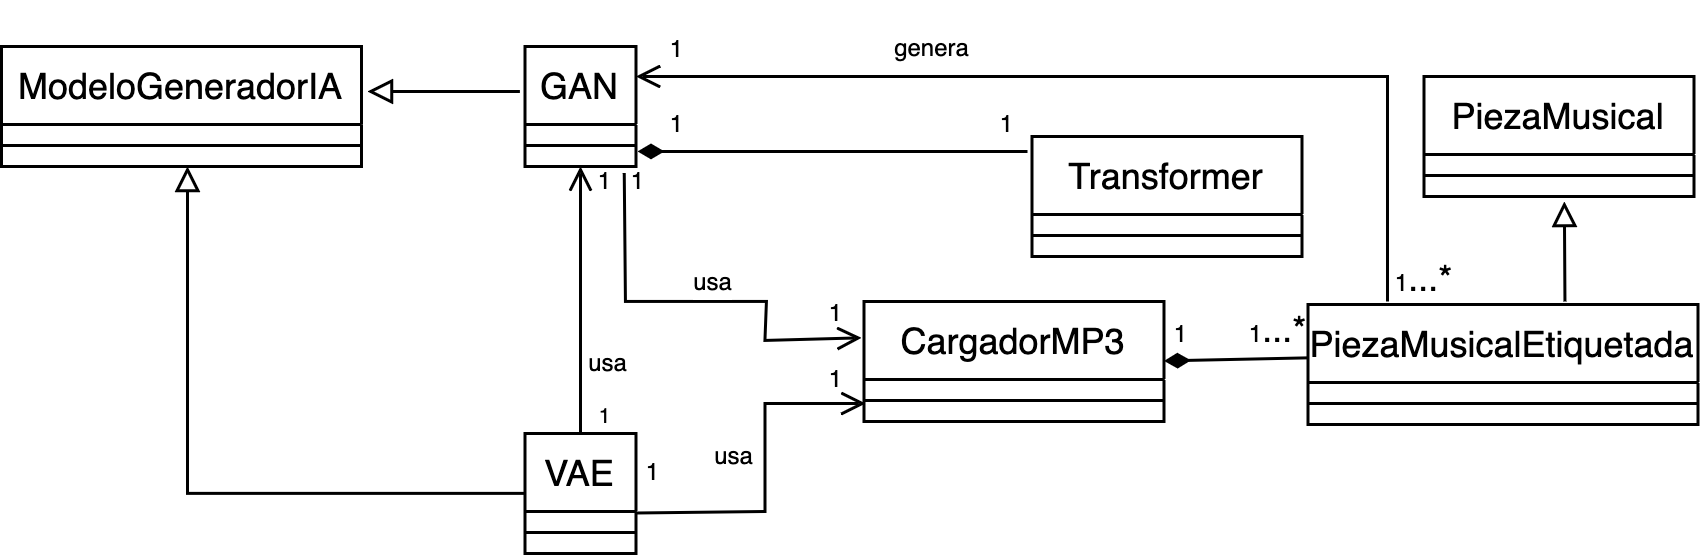
\includegraphics[width=0.9\textwidth]{images/diagrama-clases-ia.png}
    \caption{Diagrama de clases del modelo de Inteligencia Artificial.}
  \end{figure}


  \item \textbf{Diagrama de clases completo}

  \begin{figure}[H]
    \centering
    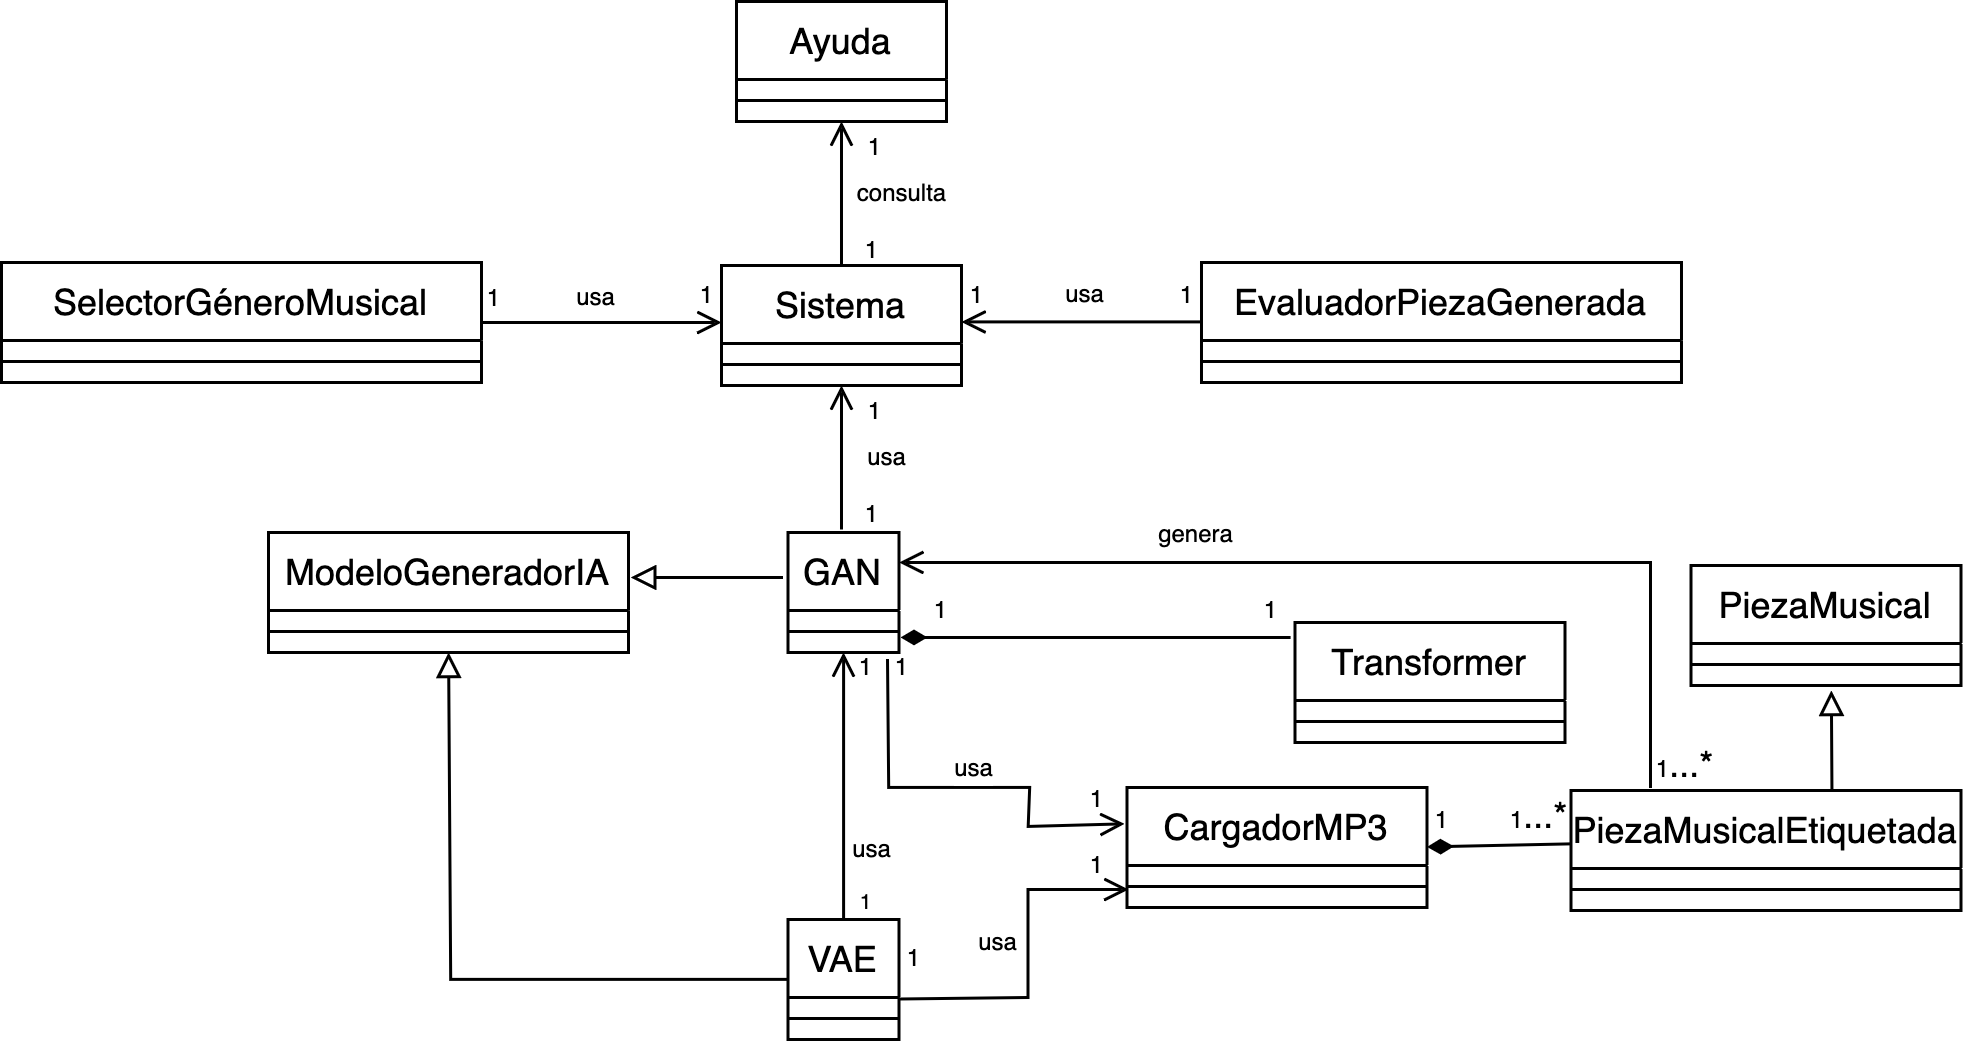
\includegraphics[width=0.9\textwidth]{images/diagrama-clases-completo.png}
    \caption{Diagrama de clases completo.}
  \end{figure}

\end{enumerate}

\subsection{Diagramas de Secuencia}

Tras la especificación del modelo de clases, el siguiente paso es crear un nuevo diagrama, en el que los dos hasta ahora mostrados, el diagrama de caso de uso y la especificación de modelo de clases, se unan y muestren una nueva visión de la información, en la que se aprecie el flujo de información entre las clases, recreando las funciones de los casos de uso, y mostrando todo esto bajo una progresión temporal. A esto se le llama Diagrama de Secuencia o Diagrama de Caso de Uso Dinámico.

En estos diagramas, la progresión temporal se despliega en el eje vertical hacia abajo, y el intercambio de datos entre clases se representa con líneas horizontales que van desde un usuario a una clase, o de una clase a otra.

Los diagramas de secuencia diseñados son los siguientes:

\begin{itemize}
    \item Creación de pieza musical.
    \item Evaluación de pieza musical.
    \item Ayuda.
\end{itemize}

Estos diagramas de secuencia dejan entrever que, en todo momento, la instanciación de objetos de clase ya se ha producido. Es decir, el sistema será un software latente e instanciable bajo demanda, que carecerá de necesidad de ser inicializado de cualquier modo.

\newpage
\subsubsection{Creación de pieza musical}

Este diagrama de secuencia representa el flujo de eventos que ocurren cuando se solicita la creación de una pieza musical.

El usuario insta al sistema, ya iniciado previamente y este le da la oportunidad de selecionar el género musical.

Tras esta selección, se produce la llamada al objeto ModeloGeneroMúsica, que devolverá una pieza musical del género requerido.

\begin{figure}[H]
  \centering
  \includesvg[width=0.9\textwidth]{images/diagrama-secuencia-generar.svg}
  \caption{Diagrama de secuencia \emph{Creación de pieza musical}.}
\end{figure}

\subsubsection{Evaluación de pieza musical}

Este diagrama de secuencia representa el flujo de eventos que ocurren cuando se emite una evaluación sobre una pieza musical generada.

El usuario insta al sistema y recorre todos los pasos a seguir para la generación de una pieza musical de un género concreto. Una vez generada, ya puede emitir su valoración. El sistema albergará dicha evaluación.

\begin{figure}[H]
  \centering
  \includesvg[width=0.9\textwidth]{images/diagrama-secuencia-eval.svg}
  \caption{Diagrama de secuencia \emph{Evaluación de pieza musical}.}
\end{figure}

\subsubsection{Consultar ayuda}

Este diagrama de secuencia representa el flujo de eventos que ocurren cuando se consulta la ayuda sobre el uso del programa.

El usuario, en cualquier momento, puede solicitar ayuda sobre el uso y funcionamiento del sistema al mismo. El sistema muestra la ayuda del programa por pantalla.

\begin{figure}[H]
  \centering
  \includesvg[width=0.5\textwidth]{images/diagrama-secuencia-ayuda.svg}
  \caption{Diagrama de secuencia \emph{Consultar ayuda}.}
\end{figure}

\subsection{Especificación de Requisitos de la Interfaz}
\label{especificacion-interfaz}
Hoy en día no se concibe un programa informático sin una interfaz gráfica de usuario.

La interfaz gráfica de usuario (GUI) brinda al usuario la capacidad de introducir y visualizar información de manera sencilla e intuitiva, y permite interaccionar con una aplicación de manera más amigable.

Además de esto, las GUI son una parte fundamental en una sociedad en que la imagen externa se antepone a la potencialidad o valor oculto tras esa máscara. De ahí la expresión: ``se mete por los ojos''. Algo que ``entra por los ojos'' es algo que cala de tal manera que tiene más probabilidad de ser aceptado que lo que no nos parece atractivo.

La GUI también permite el acceso a la informática a personas cuyas discapacidades dificultan o impiden el manejo de un antiguo programa de consola, o también da acceso a un colectivo social como es el colectivo infantil, al que permanecer delante de algo que no estimula su atención le resulta muy difícil.

Puesto que esta aplicación va orientada al uso por parte del mayor número de usuarios, con perfiles personales y profesionales distintos, la interfaz gráfica ha de ser lo más sencilla y amigable posible.

El programa se compondrá de una única ventana principal, cuyo contenido será:

\begin{itemize}
    \item Una lista de géneros musicales para seleccionar.
    \item Un botón para instar la creación de una pieza musical del género seleccionado.
    \item Un botón para dirigirse a la zona de ayuda de la ventana.
    \item Un pequeño panel que se activará cuando se recepciones el fichero con la pieza musical y que permitirá al usuario emitir una valoración entre 1 y 10 de la fidelidad de dicha pieza con el género solicitado.
\end{itemize}
\input{UML/diseño-de-clases}

\subsection{Diagrama de Paquetes}

La complejidad y tamaño de un diagrama de clases de un sistema puede llevar que la aprehensión del mismo sea compleja y difusa.

En la programación estructurada, la manera de crear un nivel más alto de abstracción es la creación de las funciones. Pero en la programación orientada a objetos, donde los datos y el procesamiento no se presentan por separado, la única manera de realizar un diagrama más inteligible y abordable, así como más sencillo de entender es el diagrama de paquetes.

Un paquete es una estructura superior, mediante la cual se agrupan varias clases, atendiendo a un criterio de empaquetamiento. El criterio usado para crear el diagrama de paquetes de este proyecto es el desempeño. Así, todas las clases utilizadas para un misma finalidad estarán agrupadas bajo un mismo paquete.

Los paquetes que se pueden extraer de la sección ``Diseño de clases'' \ref{diseño-clases} son los siguientes:

\begin{itemize}
    \item Aplicación.
    \item CargadorDataset.
    \item ModelosIA.
\end{itemize}

No existirá jerarquía entre paquetes, por lo tanto, ningún paquete contendrá a uno o varios otros.

\subsubsection{Paquete Aplicación}
Este paquete contiene las clases encargadas de conformar una aplicación informática de cara al usuario. 

Las clases contenidas son:

\begin{itemize}
  \item Sistema.
  \item SelectorGéneroMusical.
  \item EvaluadorPiezaGenerada.
  \item Ayuda.
\end{itemize}

La clase \emph{Sistema} y por ende, este paquete, verán al modelo de Inteligencia Artificial ya compilado como recurso.

\subsubsection{Paquete ModelosIA}

Este otro paquete es el encargado de contener todas las clases que intervienen en la conformación de un modelo de Inteligencia Artificial y que dará lugar a los objetos de sendos modelos utilizados en este trabajo.

La lista de clases que se pueden encontrar en este paquete son:
\begin{itemize}
  \item modeloGeneradorIA.
  \item VAE.
  \item GAN.
  \item Transformer.
\end{itemize}


\subsubsection{Paquete CargadorDataset}

Las clases que están contenidas en este paquete van orientadas al manejo del \emph{Dataset} y la abstracción de las piezas musicales en él contenidas.

Las clases que conforman este paquete son:
\begin{itemize}
  \item PiezaMusical.
  \item PiezaMusicalEtiquetada.
  \item CargadorMP3.
  \item ScriptEntrenamiento.
\end{itemize}

Se hace un especial hincapié en la clase \emph{ScriptEntrenamiento}, que si bien no está colocada en este paquete de manera trivial, pues sirve para manejar el \emph{Dataset}, también controla y gestiona todo el proceso de entrenamiento de los modelos y es la pieza central de todo el proceso previa puesta en producción, que se hace para generarlos.


\subsubsection{Diagrama general de paquetes}

\begin{figure}[H]
  \centering
  \includesvg[width=0.4\textwidth]{images/diagrama-paquetes.svg}
  \caption{Diagrama general de paquetes.}
\end{figure}

\input{UML/diseño-de-la-interfaz}
